% !TeX spellcheck = de_DE
\chapter{Optimierung}
\label{chap:optimization}
Grundsätzlich gibt es verschiedene Arten der Optimierung. In dieser Arbeit wird das sequenzielle Verfahren mit \ac{MPI} parallelisiert. Hierzu wird in Kapitel \ref{sec:parallel_strategies} die ausgewählte Parallelisierungsstrategie vorgestellt. Im Anschluss daran sind die konkreten Implementierungsdetails in Kapitel \ref{sec:parallel_implementation} erläutert. Als Testumgebung für das parallelisierte Verfahren wird ein Beowulf-Cluster erstellt, dessen Aufbau in \ref{sec:test_env_parallel} beschrieben ist. Danach wird die eigentliche Evaluation mit der \emph{Mountain Car} und \emph{Pendulum} Umgebung in Kapitel \ref{sec:test_env_parallel} vorgestellt. Neben dem Training eines \ac{KNN} für die \emph{Lunar Lander} Umgebung schließt das Kapitel mit der Zusammenfassung der Ergebnisse der Parallelisierung.

% Mehrere Arten der Optimierung, in diesem Fall soll die Parallelisierung eingesetzt werden
% !TeX spellcheck = de_DE
\section{Strategien zur Parallelisierung}
\label{sec:parallel_strategies}
Es gibt mehrere Möglichkeiten zur Umsetzung einer Parallelisierung sowie verschiedene Schwerpunkte, welche diese haben kann. Die Analyse der sequenziellen Implementierung hat gezeigt, dass die \emph{Evaluation Time} den größten Einfluss auf die Ausführungszeit hat.  Dementsprechend kann bei einer erfolgreichen Parallelisierung dieser Phase die größte Reduktion der Ausführungszeit erzielt werden. Aus diesem Grund liegt der Fokus im Weiteren hierauf. 
\begin{figure}[!h]
	\centering
	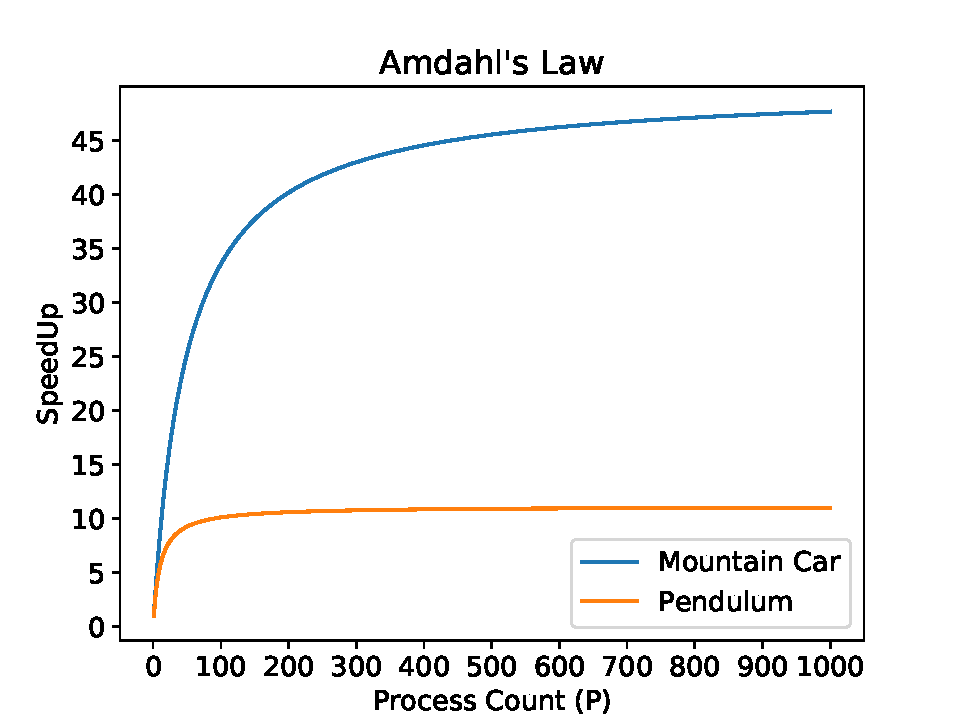
\includegraphics[width=0.5\textwidth]{./img/ahmdals_law_mountain_pendulum.pdf} 
	\caption{Durch \emph{Amdahl's Law} berechnete theoretische \emph{SpeedUp} für das \emph{Mountain Car} und \emph{Pendulum} Problem in Abhängigkeit der Anzahl an Prozessen}
	\label{fig:amdahls_law_mountain_pendulum}
\end{figure}
Mit \emph{Amdahl's Law}, welches in Kapitel \ref{subsec:basics_performance} vorgestellt ist, kann der theoretisch erreichbare \emph{SpeedUp} in Abhängigkeit von $P$ Prozessoren berechnet werden. Dies ist in Abbildung \ref{fig:amdahls_law_mountain_pendulum} dargestellt, wobei entsprechend der Analyseergebnisse angenommen wird, dass die \emph{Mountain Car} Umgebung zu $98\%$ und die \emph{Pendulum} Umgebung zu $91\%$ parallelisiert werden können. Durch die Abbildung ist ersichtlich, dass beide Probleme anfänglich mit steigender Anzahl an Prozessen sehr gute \emph{SpeedUp} Werte erzielen. Allerdings ist das Hinzufügen von weiterer Rechenleistung ab einem gewissen Punkt nicht mehr effektiv, da der Anstieg des \emph{SpeedUps} zunehmend geringer wird und schlussendlich gegen einen gewissen Wert konvergiert. Für $P \rightarrow \infty$ liegt der maximale \emph{SpeedUp} für die \emph{Mountain Car} Umgebung bei Faktor 50 und für die \emph{Pendulum} Umgebung bei Faktor $11.\overline{1}$. Auch wenn diese Ergebnisse eine ungefähre Richtlinie bieten, ist das Erreichen dieser Vorgaben in einer praktischen Umsetzung unwahrscheinlich. Durch eine hohe Anzahl an beteiligten Prozessen entsteht in der Regel ein hoher Kommunikationsaufwand, der sich negativ auf den \emph{SpeedUp} Wert auswirkt. Im Folgenden werden verschiedene Strategien zur Umsetzung einer möglichst effizienten Parallelisierung aufgezeigt und die verschiedenen Vor- und Nachteile gegeneinander abgewogen.
\\\\
Vor dem Auswählen einer geeigneten Strategie sollen die zu parallelisierenden Funktionen der \emph{Evaluation Time} analysiert werden. Im sequenziellen Verfahren wird in dieser Phase über eine Liste mit allen Agenten iteriert. Für jeden von diesen wird die Umgebung einmal zurückgesetzt und ein \ac{KNN} aus dem Genom des Agenten gebildet. Danach wird die Umgebung simuliert. Bei diesem Vorgang können beliebig viele Simulationsschritte und Aktivierungen des \ac{KNN} ausgeführt werden. 
\\\\
Ein möglicher Ansatz besteht darin, die Berechnungen in einem \ac{KNN} selbst zu parallelisieren. Dies ist eine valide Strategie, die unter anderem von Bibliotheken wie \emph{Tensorflow} und \emph{PyTorch} genutzt wird. Die einzelnen Neuronen einer Schicht können beispielsweise unabhängig voneinander aktiviert und somit auch parallelisiert werden. Zusätzlich kann eine solche Parallelisierung nicht nur mithilfe von \acp{CPU}, sondern auch auf \acp{GPU} umgesetzt werden. Diese haben in der Regel mehr unabhängige Prozessoren als normale \acp{CPU}, wodurch in vielen Fällen eine bessere Parallelisierung ermöglicht wird. Allerdings sprechen zwei Gründe gegen den Einsatz einer solchen Parallelisierungsstrategie in dieser Arbeit. Die vorgestellten Bibliotheken implementieren diese Funktionalitäten bereits, sind weit verbreitet und für verschiedene Plattformen optimiert. Zusätzlich ist es im Rahmen einer zukünftigen Erweiterung möglich, diese einfach in dieses Projekt zu integrieren. Daher ist es nicht sinnvoll, Ressourcen für die Implementierung derselben Funktionalität zu verwenden. Der zweite Grund, der gegen diese Art der Parallelisierung spricht, besteht darin, dass zwar die Aktivierungszeit des \ac{KNN}, jedoch nicht die Simulationszeit der Umgebung verkürzt wird. Diese kann je nach Komplexität des Problems sehr viel Rechenzeit in Anspruch nehmen. 
\\\\
Hier können neuroevolutionäre Algorithmen einen Vorteil bieten, da sowohl das \ac{KNN} als auch die Umgebung parallelisierbar sind. Die Idee ist, dass jeder beteiligte Prozess eine Kopie des Optimierungsproblems initialisiert. Während des Verfahrens wird jeder Agent einem Prozess zugewiesen. Dieser kann unabhängig von anderen Prozessen ein \ac{KNN} aus dem Genom erzeugen und mit diesem die gesamte Evaluation in der lokalen Umgebung durchführen. Am Ende wird nur der Fitnesswert als Ergebnis übertragen. Dieses Vorgehen bietet mehrere Vorteile. Mit dieser Strategie werden alle Funktionen der \emph{Evaluation Time} parallelisiert, inklusive des Optimierungsproblems und der Berechnungen im \ac{KNN}. In einer späteren Erweiterung kann zusätzlich eine Bibliothek wie \emph{Tensorflow} integriert werden, welche die benötigte Zeit zum Berechnen des \ac{KNN} reduziert und somit einen noch größeren \emph{SpeedUp} ermöglicht. Ein weiterer Vorteil ist die geringe Anzahl an benötigten Nachrichten. Mit $n$ Agenten müssen theoretisch nur $2 \cdot n$ Nachrichten pro Generation für die Parallelisierung der \emph{Evaluation Time} ausgetauscht werden. Hiervon wird eine Hälfte zum Verteilen der Agenten und die andere Hälfte zum Sammeln der berechneten Fitnesswerte am Ende der Evaluation benötigt. Durch diese effiziente Kommunikation ist der zusätzlich entstehende Rechenaufwand sehr gering und das Erreichen einer effizienten Parallelisierung möglich.

 



% Client Server can prevent deadlocks
% Eventually calculate ahmdals law?
% !TeX spellcheck = de_DE
\section{Implementierung}
\label{sec:parallel_implementation}
Dieses Kapitel befasst sich mit der Implementierung der bereits vorgestellten Parallelisierungsstrategie. Das Ziel ist, die Ausführungszeit des Verfahrens in einem verteilten System durch Hinzufügen von weiteren Prozessoren zu reduzieren. Bei der Umsetzung sind drei Anforderungen zu beachten. Erstens muss es mit geringem Aufwand möglich sein, die sequenzielle Implementierung durch die parallelisierte auszutauschen und umgekehrt. Zweitens muss für eine Bewertung der Effizienz der Parallelisierung ein direkter Vergleich zwischen beiden Implementierungen möglich sein. Drittens ist der Standard \ac{MPI} für die Kommunikation zu verwenden
\\\\
Für die parallelisierte Implementierung wird eine neue Klasse angelegt, die von dem in Kapitel \ref{subsubsec:library_interface} vorgestellten Interface \emph{NeatOptimizer} erbt. Da auch die sequenzielle Implementierung dieses verwendet, ist die erste Anforderung bereits erfüllt. Beide Klassen stellen dieselben Funktionen zur Verfügung und können somit jederzeit gegeneinander ausgetauscht werden. Wie in Kapitel \ref{subsubsec:library_interface} erläutert, ist die \emph{evaluate()} Funktion in diesem Interface der Einstiegspunkt für die Bibliothek und das gesamte Trainingsverfahren ist in dieser implementiert. 
\\\\
Um die zweite Anforderung zu erfüllen, ist der grundsätzliche Ablauf der \emph{evaluate()} Funktion identisch zum sequenziellen Verfahren, sodass sich nur der parallelisierte Teil des Programms unterscheidet. Zu Beginn des Trainingsverfahrens wird eine initiale Population generiert. Danach beginnt eine Schleife, in welcher die Funktionen \emph{build\_new\_generation()} und \emph{evaluate\_generation()} abwechselnd aufgerufen werden bis die Abbruchbedingung erfüllt ist. Da primär die Evaluationsphase parallelisiert wird, kann die \emph{build\_new\_generation()} Funktion vom sequenziellen Verfahren unverändert übernommen werden. In dieser sind die Phasen Selektion, Rekombination und Mutation implementiert. Die Funktion \emph{evaluate\_generation()} umfasst die Evaluation der Agenten. Da die Analyse zeigt, dass sowohl in der \emph{Mountain Car} als auch in der \emph{Pendulum} Umgebung diese Funktion den größten Einfluss auf die benötigte Rechenzeit hat, wird sie im Rahmen der Parallelisierung neu implementiert.
\\\\
Im sequenziellen Verfahren wird bei der Evaluationsphase über die Liste mit allen Agenten iteriert und für jeden nacheinander die Evaluation durchgeführt. Wie bereits in Kapitel \ref{sec:sequential_implementation} beschrieben, wird hierfür vor jedem neuen Agenten die Umgebung einmalig zurückgesetzt, das \ac{KNN} gebildet und die eigentliche Evaluation mit dem Ziel durchgeführt, am Ende einen Fitnesswert zurückzugeben. Bei der parallelisierten Implementierung werden die Agenten an alle beteiligten Prozesse verteilt, welche dann die Evaluation unabhängig voneinander durchführen. 
\\\\
Dafür muss im nächsten Schritt die Art der Kommunikation und Verteilung der Agenten festgelegt werden. In Kapitel \ref{subsec:mpi} sind die \emph{Scatter} und \emph{Gather} Funktion vorgestellt, welche sich prinzipiell für dieses Szenario anbieten. Die \emph{Scatter} Funktion verteilt die Agenten gleichmäßig auf die Prozesse und die \emph{Gather} Funktion sammelt die Ergebnisse. Zwar ist die Implementierung effizient, es ergibt sich aber ein gewichtiger Nachteil. Die \emph{Scatter} Funktion erlaubt keine dynamische Verteilungen von Lasten, was in diesem Projekt jedoch aus zwei Gründen sinnvoll ist. Der erste Grund betrifft die Evaluationszeiten, der zweite die Struktur des Clusters. Die Evaluationszeiten der Agenten unterscheiden sich in vielen Fällen. Gründe hierfür können zum einen unterschiedlich große \ac{KNN} sein, deren Berechnungszeit bzw. Aktivierungszeit variiert, zum anderen unterschiedliche Fortschritte im Optimierungsproblem. In der vorgestellten \emph{Mountain Car} Umgebung wird beispielsweise die Evaluation beendet, wenn der Agent das Ziel erreicht. In anderen Optimierungsproblemen kann die Evaluation frühzeitig abgebrochen werden, wenn ein Agent eine bestimmte Fehlentscheidung getroffen hat. Die Folge in beiden Szenarien ist, dass im Vergleich zu anderen Prozessen weniger Rechenaufwand für die Evaluation des Agenten benötigt wird. Hierdurch entsteht ein Ungleichgewicht in der Lastenverteilung. Die Folge ist, dass am Ende einer Evaluationsphase die Prozesse aufeinander warten. Somit sinkt die Effizienz und auch der erreichte \emph{SpeedUp} Wert der Parallelisierung. Auch wenn alle Agenten dieselbe Rechenlast erzeugen und diese gleichmäßig auf alle Prozesse verteilt ist, kann es in einem Beowulf Cluster zu Wartezeiten kommen. Grund hierfür ist, dass sich die Konfiguration der Hardware bei den einzelnen Geräten des Clusters und somit auch deren Leistung unterscheiden kann. Für eine gute Performance des parallelisierten Verfahrens müssen die Prozessoren bzw. Geräte des Clusters, welche mehr Rechenleistung bieten, auch proportional mehr Rechenlast zugewiesen bekommen. Dies ist mit der \emph{Scatter} Funktion nicht möglich.
\\\\
Daher soll in dieser Arbeit die \emph{Point-to-Point} Kommunikation verwendet werden, mit welcher ein dynamisches Zuteilen möglich ist. Um mögliche \emph{Deadlocks} zu vermeiden, wird eine \emph{Master-Slave} Architektur gewählt. Zu Beginn der Evaluationsphase erstellt der \emph{Master} Prozess verschiedene Arbeitspakete, welche jeweils einen zu evaluierenden Agenten enthalten. Initial wird an jeden \emph{Slave} Prozess asynchron ein Paket gesendet, welche hierauf warten. Ist dieses vollständig empfangen, wird der darin enthaltene Agent im lokalen Optimierungsproblem evaluiert und der berechnete Fitnesswert als Ergebnis an den \emph{Master} Prozess zurückgesendet. Dieser ist für die Speicherung zuständig. Danach wird überprüft, ob noch weitere Arbeitspakete zur Abarbeitung ausstehen. Ist dies der Fall, wird ein neues Pakt an den \emph{Slave} übermittelt. Erst wenn alle Pakete abgearbeitet sind, endet die Evaluation der Generation. Danach führt der \emph{Master} Prozess die erforderlichen Operationen zum Erzeugen der nächsten Generation aus. Dabei werden die gespeicherten Ergebnisse der \emph{Slaves} verwendet. Mit der neuen Generation beginnt die Evaluation erneut. Ein großer Vorteil dieses Verfahrens ist, dass Prozesse automatisch mehr Arbeitspakete zugeteilt bekommen, wenn sie entweder leistungsfähiger oder die Evaluationszeiten der Agenten kürzer sind. Zusätzlich ist die Kommunikationsstruktur strikt geregelt, sodass das Auftreten von \emph{Deadlocks} unwahrscheinlich ist.
\\\\
Für die praktische Umsetzung muss der Implementierung noch die Klasse \emph{Slave} hinzugefügt werden, welche die notwendigen Operationen enthält. Dies umfasst die Funktion \emph{setup()}, welche zum Erstellen des Optimierungsproblems bzw. der Umgebung benötigt wird und die Funktion \emph{evaluate\_agent()}. Als Parameter wird dieser Funktion ein Agent übergeben, der dann evaluiert wird. Im Rahmen dessen wird die Umgebung auf den Startzustand gesetzt, ein \ac{KNN} mit dem Genom des Agenten erzeugt und die eigentliche Evaluation in der lokalen Umgebung durchgeführt. Die Funktion gibt am Ende den Fitnesswert sowie optionale Zusatzinformationen der Umgebung zurück. Insgesamt entspricht diese Funktionalität der des sequenziellen Verfahrens. Die \emph{setup()} Funktion erstellt die Umgebung, benötigt aber einen anderen Implementierungsansatz als die \emph{evaluate\_agent()} Funktion. Der Grund hierfür ist der Parameter. Ein Agent enthält nur Daten, aber keine Funktionalität. Aus diesem Grund kann er einfach mit \ac{MPI} serialisiert und versendet werden. Ein Optimierungsproblem hingegen kann eine komplexe Klasse mit unterschiedlichen Funktionen sein, die unter Umständen nicht serialisiert werden können. Zusätzlich sind in der implementierte Bibliothek keine Informationen über die Funktionalitäten, Architektur und den internen Zustand der Umgebung enthalten. Grund hierfür ist, dass neue Optimierungsprobleme von Nutzern jederzeit hinzugefügt werden können und es diesbezüglich keine Einschränkungen geben soll. Daher kann das Optimierungsproblem nicht mit \ac{MPI} serialisiert werden. Stattdessen wird der Umstand genutzt, dass der Programmcode auf jedem beteiligten Gerät bzw. Prozessor vorliegen muss. Beim Starten einer \ac{MPI} Anwendung wird auf jedem beteiligten Prozess eine Kopie des Programms ausgeführt. Hierbei kann jeder Prozess auf Basis des zugewiesenen Rangs entscheiden, ob er die Funktion eines \emph{Masters} oder \emph{Slaves} einnimmt. Der \emph{Master} führt die notwendigen Operationen zum Erstellen der initialen Generation durch und startet den Optimierungsprozess. Die \emph{Slaves} greifen auf das im Programmcode vorliegende Optimierungsproblem zu und initialisieren es. Bei einem solchen Vorgehen ist es nicht erforderlich, das Optimierungsproblem zu serialisieren und zu versenden.
\\\\
Der letzte hier vorgestellte Implementierungsaspekt bezieht sich auf die Umsetzung der \emph{Point-to-Point} Kommunikation. Hierfür wird das Paket \emph{mpi4py} verwendet, welches eine Python Schnittstelle zum Nutzen von \ac{MPI} Funktionen bietet. Das Paket selbst ist \emph{open source} verfügbar und im Vergleich zu anderen Implementierungen weit verbreitet. Zusätzlich bietet es eine gute Performance, welche in Quelle \cite{dalcin2008mpi} gemessen wurde, und ist nur geringfügig langsamer als eine Implementierung in der Programmiersprache C. Ein letzter entscheidender Vorteil sind verschiedene in der Bibliothek implementierte high-level Funktionen. Diese ermöglichen unter anderem das einfache Umsetzen der oben beschriebenen \emph{Master-Slave} Kommunikation. Diese Funktionen werden in dieser Arbeit für die Kommunikation verwendet.

% !TeX spellcheck = de_DE
\section{Testumgebung} % TODO ABBILDUNG
\label{sec:test_env_parallel}
Das nächste Kapitel befasst sich mit der Evaluation des parallelisierten Verfahrens und führt einen Vergleich mit der sequenziellen Implementierung durch. Zuvor wird in diesem Kapitel auf die verwendete Testumgebung sowie die Installation der notwendigen Software eingegangen. 
\\\\
Der größte Unterschied dieser Testumgebung im Vergleich zu der des sequenziellen Verfahrens besteht darin, dass das parallelisierte Verfahren nicht auf einem Raspberry Pi 4, sondern auf einem Beowulf-Cluster ausgeführt wird, welcher schematisch in Abbildung (TODO ABBILDUNG) dargestellt ist. Insgesamt stehen zehn identisch konfigurierte Raspberry Pi 4 \emph{Nodes} zur Verfügung. Die Hardware von diesen entspricht der Beschreibung in Kapitel \ref{sec:analysis_testsetup}. Somit besitzt der entstehende Cluster die zehnfache Rechenleistung im Vergleich zu der Testumgebung des sequenziellen Verfahrens.
\\\\
Entsprechend  der in Kapitel \ref{subsubsec:beowulf_cluster} definierten Anforderungen an einen Beowulf Cluster ist jeder Raspberry Pi durch eine Ethernet Verbindung mit einem Netzwerkswitch verbunden. Die maximale Bandbreite für jeden Raspberry Pi beträgt ein Gigabit. Hinsichtlich der Software wird das bisher verwendete Betriebssystem sowie alle Softwarepakete von der sequenziellen Testumgebung übernommen. Allerdings werden für die Kommunikation im Beowulf Cluster noch weitere Softwarekomponenten benötigt. Zuerst wird das MPICH installiert. Wie in Kapitel \ref{subsec:mpi} beschrieben, ist dies eine weit verbreitete \emph{open source} Implementierung des \ac{MPI} Standards. Zusätzlich wird in der Python Umgebung das bereits vorgestellte Paket \emph{mpi4py} installiert, welches den Zugriff auf \ac{MPI} Funktionen aus Python ermöglicht. Ab diesem Zeitpunkt kann die Implementierung lokal getestet werden. Dennoch kann das Verfahren noch nicht auf dem gesamten Beowulf Cluster ausgeführt werden, da die einzelnen \emph{Nodes} noch nicht miteinander kommunizieren können. Hierfür wird zusätzlich das \ac{SSH} Protokoll benötigt. Beim Beginn der Ausführung eines \ac{MPI} Programms wird eine \ac{SSH} Verbindung von jedem teilnehmenden Prozess zu allen anderen erstellt, über welche dann die spätere \ac{MPI} Kommunikation erfolgt. Für die Authentifizierung im \ac{SSH} Protokoll wird in diesem Fall ein asymmetrischer kryptographischer Schlüssel benötigt. Auf jedem Raspberry Pi wird hiervon einer erzeugt, welcher aus einem öffentlichen und privaten Teil besteht. Von jedem Raspberry Pi wird der öffentliche Teil des Schlüssels auf den anderen Geräten des Clusters hinterlegt, sodass eine Authentifizierung ohne Passworteingabe möglich ist.
\\\\
Nach Konfiguration des \ac{SSH} Protokolls kann das Optimierungsverfahren gestartet werden, sobald der Programmcode auf allen beteiligten Geräten vorliegt. Prinzipiell kann dieser manuell an jede einzelne \emph{Node} verteilt werden. Dies ist zeitaufwendig und nicht für die aktive Entwicklung geeignet, daher wird in dieser Testumgebung eine automatisierte Lösung angestrebt. Wie in Kapitel \ref{subsubsec:beowulf_cluster} beschrieben, kann die \emph{Master Node} eines Beowulf Clusters verschiedene organisatorische Aufgaben übernehmen. In diesem Projekt gehört hierzu unter anderem eine Schnittstelle zu den externen Umgebungen, über welche das Optimierungsverfahren gestartet werden kann. Zusätzlich wird für die automatisierte Verteilung des Programmcodes ein Ordner im Netzwerk des Beowulf Clusters freigegeben. Dieser kann von den \emph{Slaves} lokal hinzufügt werden. Der Programmcode bzw. die benötigten Dateien müssen auf dem \emph{Master} im freigegebenen Ordner vorhanden sein. Mit entsprechender Standardsoftware kann eine automatisierte Verteilung und Synchronisation der Dateien umgesetzt werden. Änderungen sind direkt auf allen \emph{Slaves} verfügbar und fehlende oder inkonsistente Dateien werden vermieden.

% !TeX spellcheck = de_DE
\section{Evaluation}
Nachdem die Parallelisierung der Evaluationsphase durchgeführt und die Testumgebung spezifiziert ist, wird in diesem Kapitel die Performance des Verfahrens gemessen. Die hierbei erhaltenen Ergebnisse werden mit denen der sequenziellen Implementierung verglichen. Im letzten Schritt wird eine Bewertung bezüglich der Effizienz und des \emph{SpeedUps} abgegeben.

\subsection{Mountain Car}
\label{subsec:mountain_car_optimzation}
Das parallelisierte Verfahren wird zuerst in der \emph{Mountain Car} Umgebung getestet, die aus Kapitel \ref{subsec:analysis_mountain_car} bekannt ist. Mit dem Ziel, einen einfachen Vergleich zwischen der sequenziellen und parallelisierten Implementierung zu ermöglichen, wird die zuvor verwendete Konfiguration des Verfahrens vollständig übernommen. Selbiges gilt für den \emph{Seed}. Bei korrekter Implementierung des parallelisierten Verfahrens werden dieselben Zwischenergebnisse nach jeder Generation generiert und das finale Ergebnis stimmt mit dem des sequenziellen Verfahrens überein. Somit kann keine Implementierung einen zeitlichen Vorteil erlagen, der durch bessere Agenten oder kürzere Evaluationszeiten entsteht. Beide Implementierungen werden dieselben Berechnungen und Evaluationen durchführen.
\begin{figure}[!h]
	\centering
	\begin{minipage}[]{0.49\textwidth}
		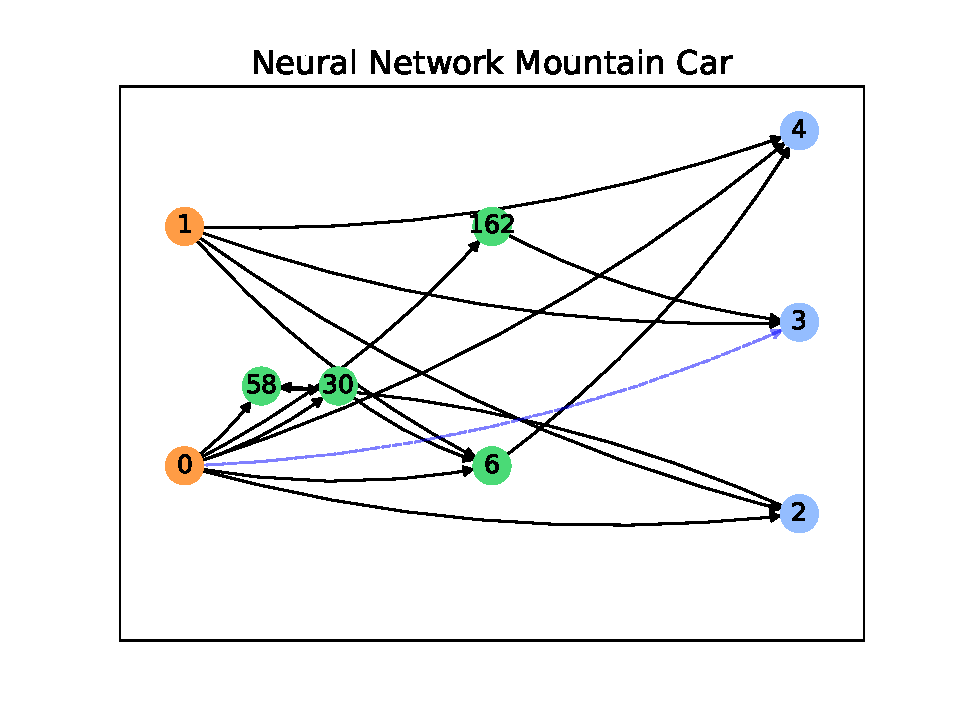
\includegraphics[width=1.0\textwidth]{./img/mountain_car_single/mountain_car_neural_network.pdf} 
	\end{minipage}
	\hfill
	\begin{minipage}[]{0.49\textwidth}
		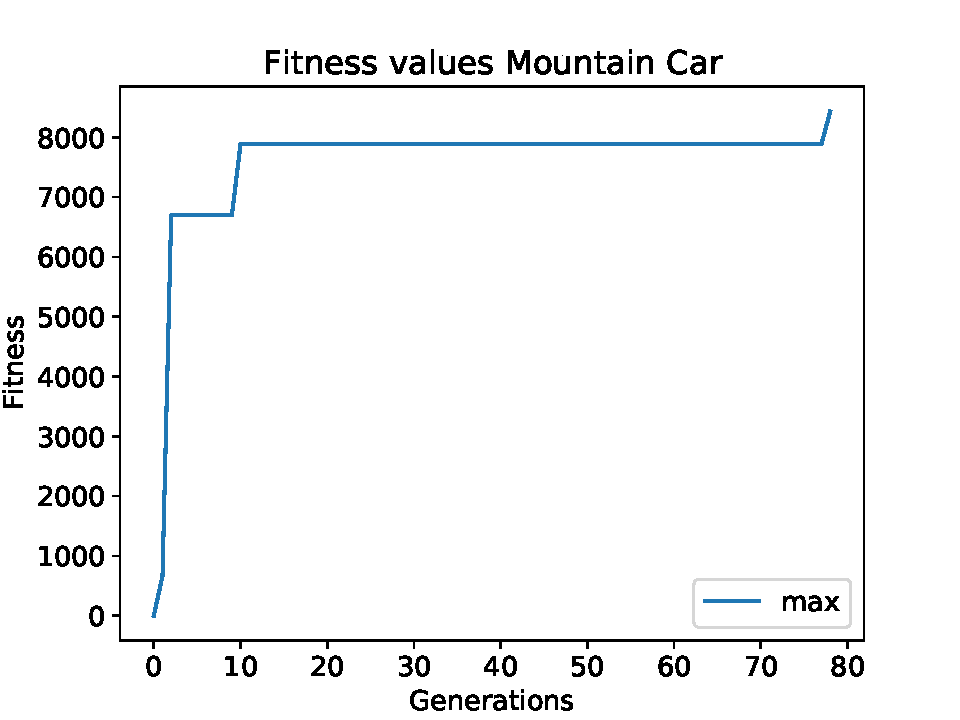
\includegraphics[width=1.0\textwidth]{./img/mountain_car_single/1413_fitness_1core_1pi.pdf} 
	\end{minipage}
	\caption{Links die Lösung für das Mountain Car Problem, rechts die dazugehörigen Fitnesswerte pro Generation mit 10 Prozessen}
	\label{fig:mountain_car_10core_neural_network_and_fitness}
\end{figure}
\begin{figure}[!h]
	\centering
	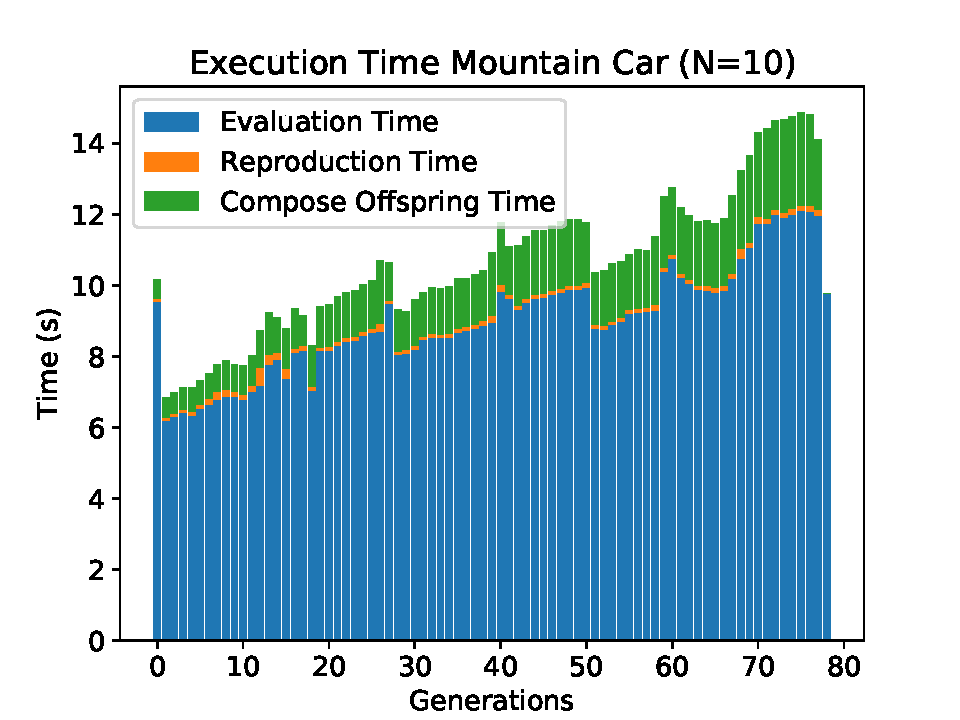
\includegraphics[width=0.7\textwidth]{./img/mountain_car_analysis/1413_time_10cores_10pis.pdf} 
	\caption{Ausführungszeit des \emph{Mountain Car} Problems auf 10 \emph{Raspberry Pis} mit 10 Prozessen}
	\label{fig:mountain_car_time_10cores_10pi}
\end{figure}
\\\\
Im ersten Durchlauf wird der parallelisierte Algorithmus mit zehn Prozessen auf zehn Raspberry Pis ausgeführt. Das Verfahren ist so konfiguriert, dass auf jedem Raspberry Pi ein Prozess gestartet wird. Abbildung \ref{fig:mountain_car_10core_neural_network_and_fitness} zeigt das hierbei entstandene \ac{KNN} und den maximal erreichten Fitnesswert. Beide Darstellungen sind identisch mit denen des sequenziellen Verfahrens. Da auch die restlichen Zwischenergebnisse übereinstimmen, wie beispielsweise die Anzahl an verschiedenen Spezies pro Generation, ist die Anforderung bezüglich des \emph{Seeds} erfüllt. Sowohl die parallelisierte als auch die sequenzielle Implementierung führen dieselben Rechenschritte aus, wodurch ein direkter Vergleich der Laufzeiten möglich ist. Die Ausführungszeit für die vorgestellte Konfiguration ist in Abbildung  \ref{fig:mountain_car_time_10cores_10pi} dargestellt. Wie beim sequenziellen Verfahren wird diese in die Phasen \emph{Evaluation Time}, \emph{Reproduction Time} und \emph{Compose Offspring Time} unterteilt. Grundsätzlich ist festzustellen, dass die insgesamt benötigte Laufzeit stark verringert ist. Mit zehn Prozessen in der vorgestellten Konfiguration sinkt die durchschnittliche Rechenzeit auf ungefähr $10.5$ Sekunden pro Generation. Die sequenzielle Implementierung hat im Vergleich dazu etwa $80$ Sekunden pro Generation benötigt. Für die gesamte Ausführungszeit des Verfahrens bedeutet dies, dass das parallelisierte Verfahren bereits nach $14$ Minuten beendet ist. Im Vergleich zur Laufzeit der sequenziellen Implementierung mit $105$ Minuten ist das parallelisierte Verfahren $91$ Minuten schneller.
\\\\
Eine Besonderheit des Graphen zeigt sich in der ersten Generation. In dieser ist die Ausführungszeit der \emph{Evaluation Time} vergleichsweise hoch. Der Grund hierfür ist, dass das Starten und Initialisieren der beteiligten Prozesse Zeit benötigt, welche die Evaluation der Agenten verzögert. Da dies im Rahmen der \emph{Evaluation Time} erfasst wird, erhöht sich die gemessene Ausführungszeit in der ersten Generation. Für die nachfolgenden Generationen trifft dies nicht mehr zu, da die Initialisierung nur einmalig zu Beginn erfolgt. Eine weitere Besonderheit betrifft die Form des Graphen. Wie bei der sequenziellen Implementierung gibt es auch in der parallelisierten Implementierung Generationen, in denen die Ausführungszeit stark sinkt oder ansteigt. Mögliche Gründe hierfür sind in Kapitel \ref{subsec:analysis_mountain_car} erörtert. Bei einem direkten Vergleich der Ausführungszeiten ist festzustellen, dass diese Änderungen meistens in denselben Generationen auftreten. Diese Eigenschaft ist wichtig, da ein Vergleich der Laufzeiten nur möglich ist, wenn die Messergebnisse, von kleinen Abweichungen abgesehen, konsistent sind. Diese Eigenschaft kann zusätzlich mit der \emph{Reproduction Time} und \emph{Compose Offspring Time} verifiziert werden. Diese Phasen sind nicht parallelisiert und daher sollte die Ausführungszeit identisch sein. Insgesamt sind die gemessenen Laufzeiten in diesen Phasen etwas höher als bei der sequenziellen Implementierung. Über alle $78$ Generationen entsteht eine Differenz von ungefähr $5$ Sekunden beziehungsweise $4\%$. Diese Unterschiede können beispielsweise durch Hintergrundprozesse im Betriebssystem entstehen, auf welche kein Einfluss genommen werden kann. Da die Abweichungen insgesamt gering sind, kann dennoch ein Vergleich der Laufzeiten vorgenommen werden. Die letzte zu nennende Eigenschaft bezüglich der Abbildung \ref{fig:mountain_car_time_10cores_10pi} ist der prozentuale Anteil der \emph{Reproduction Time} und \emph{Compose Offspring Time}. Bei der sequenziellen Implementierung haben diese beiden Phasen nur etwa $2\%$ der Ausführungszeit in Anspruch genommen. Im aktuellen Testdurchlauf sind dies $15\%$, da durch die Parallelisierung der Anteil der \emph{Evaluation Time} sinkt. Aufgrund \emph{Amdahl's Law} ist anzunehmen, dass durch das Hinzufügen von weiteren Prozessen der prozentuale Anteil der \emph{Reproduction Time} und \emph{Compose Offspring Time} weiter ansteigt.
\begin{figure}[!h]
	\centering
	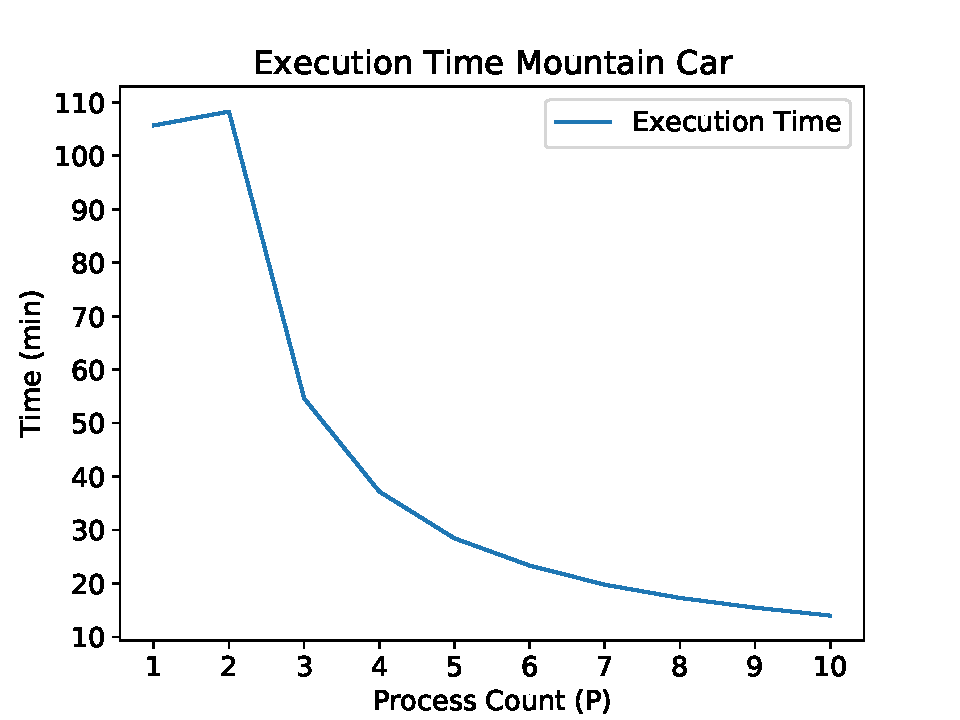
\includegraphics[width=0.7\textwidth]{./img/mountain_car_analysis/time_mountain_car_1_10.pdf} 
	\caption{Ausführungszeit des parallelisierten Verfahrens in der \emph{Mountain Car} Umgebung in Abhängigkeit zur Prozessanzahl}
	\label{fig:execution_time_mountain_car_1_10}
\end{figure}
\\\\
Für eine vollständige Bewertung des parallelisierten Verfahrens werden die in Kapitel \ref{subsec:basics_performance} vorgestellten Metriken \emph{SpeedUp} und Effizienz benötigt. Für eine bessere Einordnung der Ergebnisse werden diese nicht nur für die oben vorgestellte Konfiguration mit zehn Prozessen, sondern auch für Testdurchläufe mit zwei bis neun Prozessen berechnet. Diese werden im Folgenden mit derselben Konfiguration durchgeführt. Die hierbei entstehenden \ac{KNN} und Fitnesswerte sind identisch mit den vorherigen und sind daher nicht abgebildet. Die benötigte Ausführungszeit für das gesamte Verfahren in Abhängigkeit zur Anzahl an Prozessen ist in Abbildung \ref{fig:execution_time_mountain_car_1_10} dargestellt. Eine Besonderheit hierbei ist, dass die benötigte Ausführungszeit mit zwei Prozessen länger ist als die mit einem Prozess. Der Grund hierfür liegt in der gewählten \emph{Master-Slave} Architektur des parallelisierten Verfahrens. Mit einem Prozess wird das sequenzielle und andernfalls das parallelisierte Verfahren ausgeführt. Werden genau zwei Prozesse verwendet, gibt es einen \emph{Master} und einen \emph{Slave}. In diesem Fall ist die Ausführung langsamer als beim sequenziellen Verfahren, da der \emph{Master} im Rahmen der Parallelisierung nur die Kommunikation koordiniert, selbst aber keine Aufgabenpakete abarbeitet. Der \emph{Slave} führt alleine die Evaluation der Agenten durch. Dafür benötigt er dieselbe Zeit wie das sequenzielle Verfahren. Hinzu kommt der benötigte Kommunikationsaufwand für das Verteilen der Agenten und Sammeln von Fitnesswerten. Aufgrund der hierfür aufgewendeten Zeit ist das parallelisierte Verfahren mit zwei Prozessen langsamer als das sequenzielle Verfahren. Mit drei oder mehr beteiligten Prozessen sinkt die Ausführungszeit kontinuierlich. 
\begin{figure}[!h]
	\centering
	\begin{minipage}[]{0.49\textwidth}
		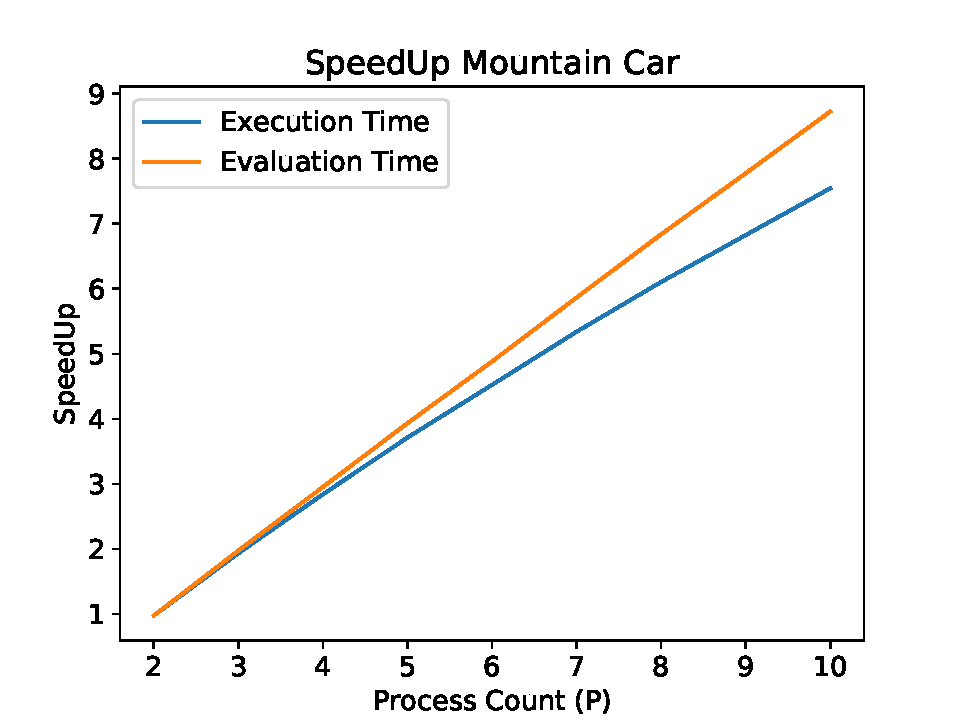
\includegraphics[width=1.0\textwidth]{./img/mountain_car_analysis/mountain_car_speedup_2_10.pdf} 
	\end{minipage}
	\hfill
	\begin{minipage}[]{0.49\textwidth}
		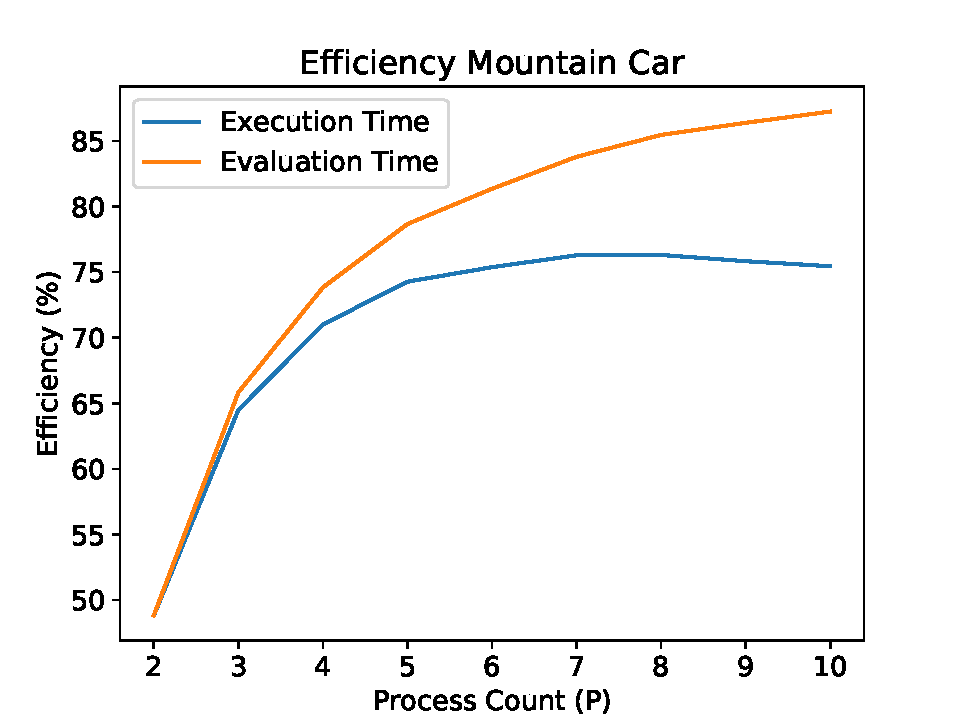
\includegraphics[width=1.0\textwidth]{./img/mountain_car_analysis/efficecny mountain_car_2_10.pdf} 
	\end{minipage}
	\caption{Links der \emph{SpeedUp}, rechts die dazugehörigen Effizienzwerte für die \emph{Mountain Car} Umgebung in Abhängigkeit zur Prozessanzahl}
	\label{fig:mountain_car_2_10_efficiency_speedup}
\end{figure}
\\\\
Anhand der Ausführungszeiten wird der \emph{SpeedUp} und die Effizienz des parallelisierten Verfahrens gemessen, welche eine Bewertung der Implementierung ermöglichen. Abbildung \ref{fig:mountain_car_2_10_efficiency_speedup} zeigt links die erreichten \emph{SpeedUps} und rechts die dazugehörigen Effizienzwerte in Abhängigkeit zur Anzahl an verwendeten Prozessen. In beiden Graphen sind jeweils die Metriken für die Evaluationsphase und das gesamte Verfahren dargestellt. Beim Testdurchlauf mit zehn Prozessen ist das parallelisierte Verfahren ungefähr um den Faktor $7.6$ schneller als das sequenzielle Verfahren. Dieses Ergebnis ist grundsätzlich höher als bei den vorherigen Testdurchläufen mit weniger Prozessen, entspricht aber nicht der Vorhersage von \emph{Amdahl's Law}. Laut diesem liegt der maximal erreichbare \emph{SpeedUp} mit zehn Prozessen in einem zu $98\%$ parallelisierbaren Programm bei ungefähr $8.5$. Durch die gewählte \emph{Master-Slave} Kommunikationsarchitektur ist zwischen dem erwarteten und tatsächlich erhaltenen Wert eine Differenz von $0.9$. Wie bereits beschrieben, unterstützt der \emph{Master} die \emph{Slaves} nicht bei der Evaluation, wird aber dennoch bei den Berechnungen berücksichtigt. Wird nur die Anzahl der \emph{Slave} Prozesse bei der Berechnung von \emph{Amdahl's Law} verwendet, ergibt sich ein maximaler \emph{SpeedUp} von $7.8$. Die restliche Differenz von $0.2$ entsteht durch den Kommunikationsaufwand. 
\begin{figure}[!h]
	\centering
	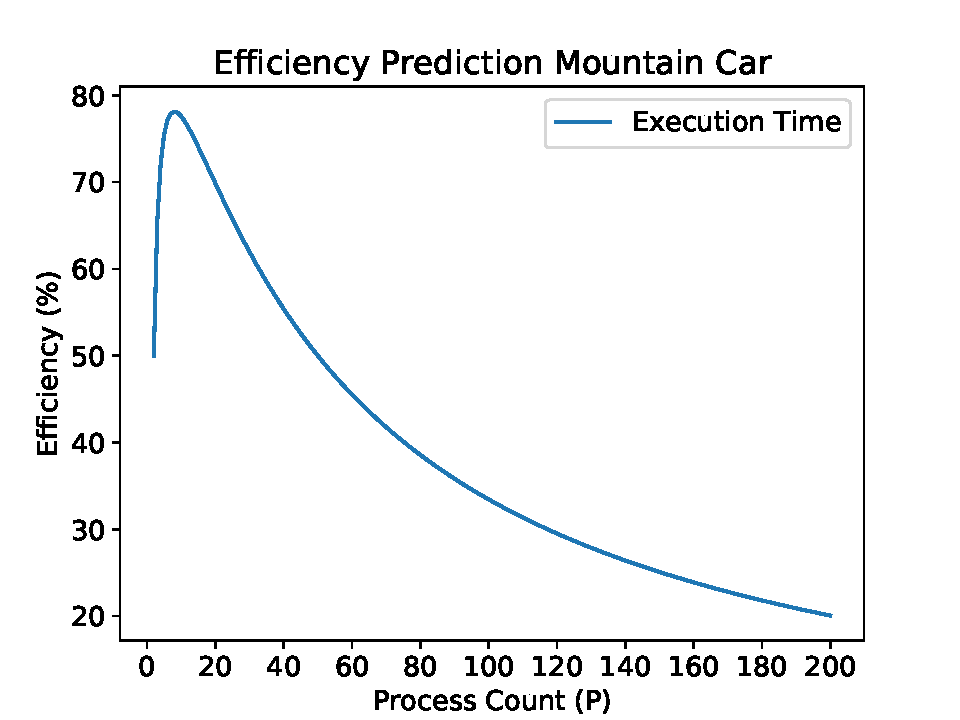
\includegraphics[width=0.7\textwidth]{./img/mountain_car_analysis/mountain_car_efficiency_prediction.pdf} 
	\caption{Erwartete Effizienz in der \emph{Mountain Car} Umgebung in Abhängigkeit zur Anzahl an Prozessen}
	\label{fig:mountain_car_efficiency_predidction}
\end{figure}
\\\\
Die in Abbildung \ref{fig:mountain_car_2_10_efficiency_speedup} rechts dargestellten Effizienzwerte beurteilen den \emph{SpeedUp} anhand der Prozessanzahl. Initial erzielt das parallelisierte Verfahren mit zwei Prozessen aufgrund der \emph{Master-Slave} Architektur eine geringe Effizienz. Mit je einem \emph{Master} und \emph{Slave} wird entsprechend der Abbildung \ref{fig:execution_time_mountain_car_1_10} eine etwas höhere Ausführungszeit im Vergleich zur sequenziellen Implementierung benötigt. Daher liegt der \emph{SpeedUp} bei ungefähr $0.98$. Entsprechend der Formel aus Kapitel \ref{subsec:basics_performance} ergibt die Berechnung der Effizienz einen Wert von $49\%$. Beim Hinzufügen weiterer Prozesse sinkt der Einfluss des \emph{Masters} auf das Ergebnis und die Effizienz steigt. Mit sechs bis zehn Prozessen wird ein Wert von über $75\%$ erreicht. Aufgrund des Graphen und \emph{Amdahl's Law} ist davon auszugehen, dass der Wert nicht weiter steigen, sondern durch Hinzufügen weiterer Prozesse letztendlich sinken wird. Abbildung \ref{fig:mountain_car_efficiency_predidction} zeigt die erwarteten Effizienzwerte für die \emph{Mountain Car} Umgebung mit einer \emph{Master-Slave} Architektur, wobei die Werte mit \emph{Amdahl's Law} berechnet worden sind. Auch in diesem Fall steigt die Effizienz anfangs stark an. Der höchste Wert von ungefähr $78\%$ wird mit acht Prozessen erreicht. Dies entspricht etwa dem tatsächlich erhaltenen Ergebnis. Hierbei wird die höchste Effizienz von $76\%$ ebenfalls mit acht Prozessen erreicht. Der Grund für das starke Absinken der Effizienz im weiteren Verlauf ist darin begründet, dass der \emph{SpeedUp} durch den sequenziellen Anteil von \emph{Amdahl's Law} immer gegen einen bestimmten Wert konvergiert. Die niedrigen Effizienzwerte entstehen, da der \emph{SpeedUp} nicht proportional zur Anzahl der Prozesse ansteigt.
\\\\
Es ist möglich, den \emph{SpeedUp} und die Effizienz nur für die parallelisierte \emph{Evaluation Time} zu berechnen, sodass der sequenzielle Teil des Verfahrens keinen Einfluss auf das Ergebnis hat. Die Ergebnisse hiervon sowie die des gesamten Verfahrens sind in Abbildung \ref{fig:mountain_car_2_10_efficiency_speedup} dargestellt. Der \emph{SpeedUp} der \emph{Evaluation Time} ist nahezu linear. Mit neun \emph{Slaves} bzw. zehn Prozessen wird ein \emph{SpeedUp} von $8.7$ erreicht. Diese guten Ergebnisse spiegeln sich in der Effizienz wieder. Diese ist anfänglich durch die \emph{Master-Slave} Architektur bei $49\%$, steigt aber stetig an. Mit zehn Prozessen liegt sie bei $87\%$. Prinzipiell kann der Wert weiter ansteigen, da der Einfluss des \emph{Masters} auf das Ergebnis mit zunehmender Prozessanzahl sinkt. Dennoch ist aufgrund der entstehenden Kommunikationszeit keine Effizienz von $100\%$ möglich. Bleibt bei der Effizienzberechnung der \emph{Master} Prozess unberücksichtigt, werden Ergebnisse zwischen $97\%$ und fast $99\%$ erreicht. Dies entspricht nahezu dem idealen Wert.

\subsection{Pendulum}
In diesem Kapitel wird die \emph{Pendulum} Umgebung mit dem parallelisierten Verfahren evaluiert und bewertet. Zusätzlich erfolgt ein Vergleich mit den Ergebnissen des vorherigen Kapitels. Hierzu wird das Optimierungsproblem zunächst in verschiedenen Testdurchläufen mit zwei bis zehn Prozessen optimiert und jeweils die \emph{Evaluation Time}, \emph{Reproduction Time} und \emph{Compose Offspring Time} erfasst. Die Konfiguration und der \emph{Seed} werden vom sequenziellen Verfahren übernommen, sodass alle Testdurchläufe dieselben Lösungen produzieren und ein Vergleich der Implementierungen möglich ist. Wie bei der \emph{Mountain Car} Umgebung, wird von jedem Raspberry Pi maximal ein Prozess ausgeführt. 
\begin{figure}[!htb]
	\centering
	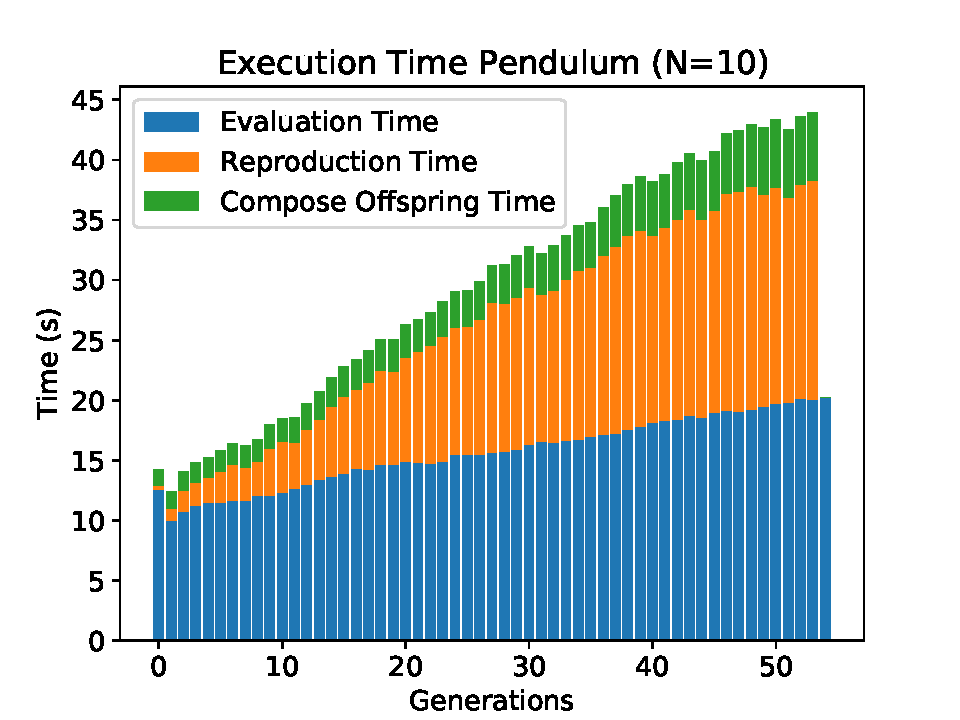
\includegraphics[width=0.7\textwidth]{./img/pendulum_analysis/pendulum_time_1_10core_10pi.pdf} 
	\caption{Ausführungszeit des \emph{Pendulum} Problems auf 10 \emph{Raspberry Pis} mit 10 Prozessen}
	\label{fig:pendulum_time_10cores_10pi}
\end{figure}
\\\\
Die Ergebnisse zeigen, dass die Fitnesswerte und die finalen \ac{KNN} identisch mit denen des sequenziellen Verfahrens sind, daher wird auf eine Abbildung verzichtet. Der Schwerpunkt der Analyse liegt auf den Ausführungszeiten. Diese sind von dem zuletzt durchgeführten Test mit zehn Prozessen in Abbildung \ref{fig:pendulum_execution_time_1_10} dargestellt. Wie bei der \emph{Mountain Car} Umgebung ist die \emph{Evaluation Time} der ersten Generation höher als die der zweiten. Der Grund hierfür liegt in der Initialisierung der einzelnen Prozesse. Die gesamte Ausführungszeit in diesem Test beträgt $27$ Minuten. Verglichen mit der Ausführungszeit der sequenziellen Implementierung von 138 Minuten ist dies eine Zeitersparnis von $111$ Minuten. Zuletzt ist bezüglich dieses Graphen hervorzuheben, dass die \emph{Evaluation Time} im Verlauf der Generationen nur leicht ansteigt und insgesamt $53\%$ der Ausführungszeit ausmacht. Der Anteil der beiden anderen Phasen ist anfänglich gering, steigt aber stark an und benötigt zusammen in den letzten Generationen mehr Zeit als die eigentliche Evaluation. Wie bereits beim sequenziellen Verfahren beschrieben, ist die hohe Anzahl an verschiedenen Spezies der Grund für die vergleichsweise hohe \emph{Reproduction Time}.
\begin{figure}[!htb]
	\centering
	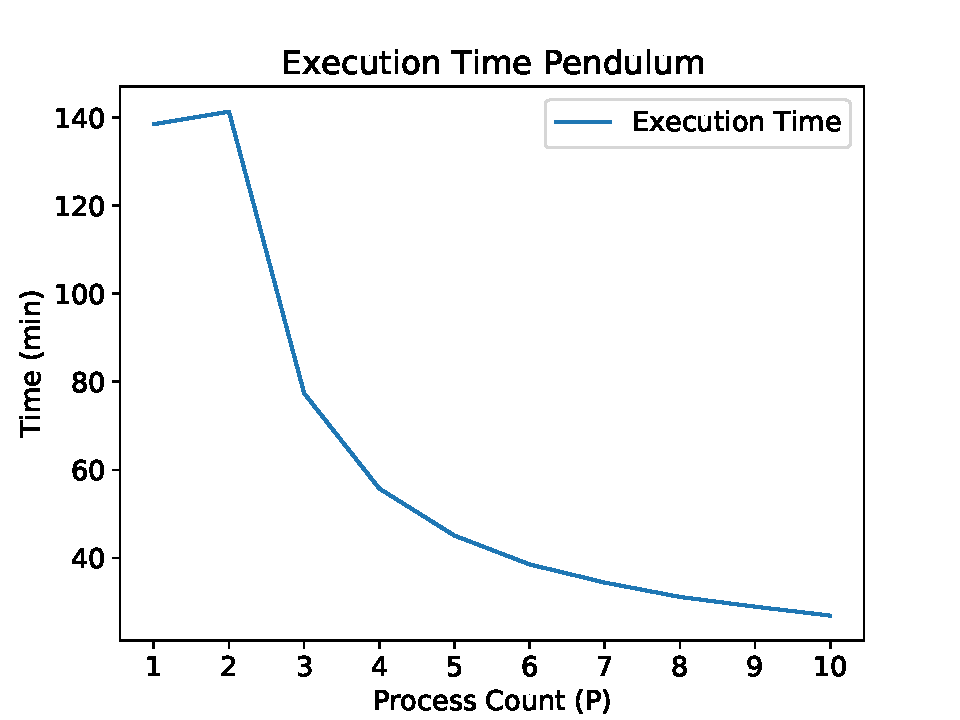
\includegraphics[width=0.7\textwidth]{./img/pendulum_analysis/pendulum_execution_1_1_10.pdf} 
	\caption{Ausführungszeit des parallelisierten Verfahrens in der \emph{Pendulum} Umgebung in Abhängigkeit zur Prozessanzahl}
	\label{fig:pendulum_execution_time_1_10}
\end{figure}
\\\\
Als nächstes wird der Verlauf der gesamten Ausführungszeit in Abhängigkeit zur Anzahl an Prozessen betrachtet. Diese sind in Abbildung \ref{fig:pendulum_execution_time_1_10} dargestellt. Prinzipiell ähnelt der Graph dem der \emph{Mountain Car} Evaluation. Mit zwei Prozessen steigt die Ausführungszeit im Vergleich zum sequenziellen Verfahren an. Wie in Kapitel \ref{subsec:mountain_car_optimzation} beschrieben, ist der Grund hierfür die gewählte \emph{Master-Slave} Architektur. Mit steigender Anzahl an Prozessen nimmt die Ausführungszeit kontinuierlich ab. Gegen Ende wird die Zeitersparnis mit zunehmender Anzahl an Prozessen immer geringer. Grund hierfür sind die sequenziellen Phasen des Verfahrens. 
\begin{figure}[!htb]
	\centering
	\begin{minipage}[]{0.49\textwidth}
		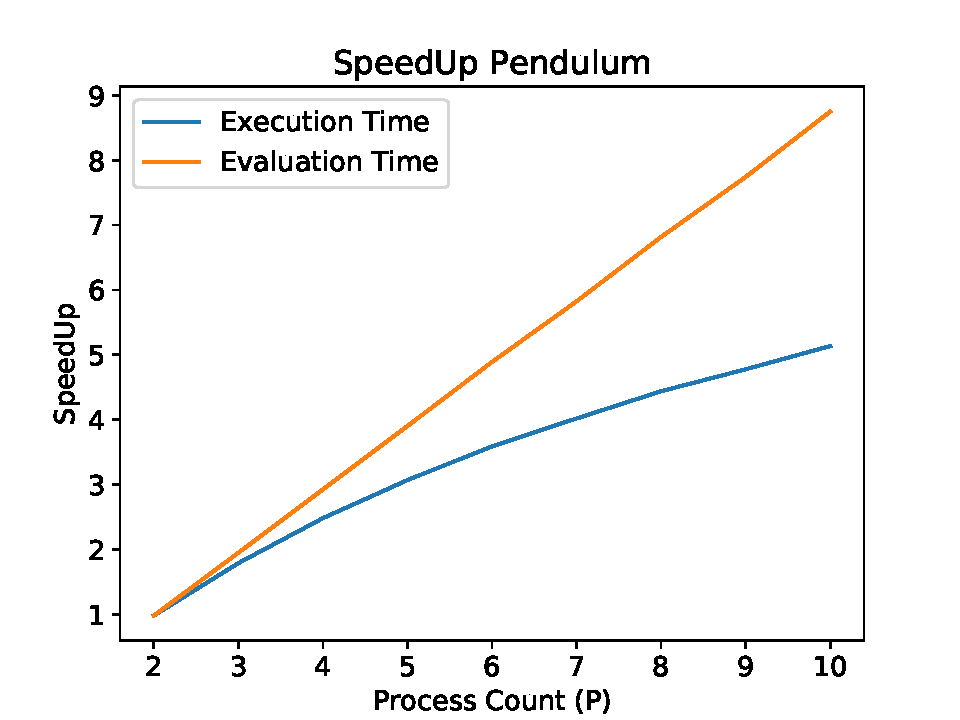
\includegraphics[width=1.0\textwidth]{./img/pendulum_analysis/pendulum_speedup1_2_10.pdf} 
	\end{minipage}
	\hfill
	\begin{minipage}[]{0.49\textwidth}
		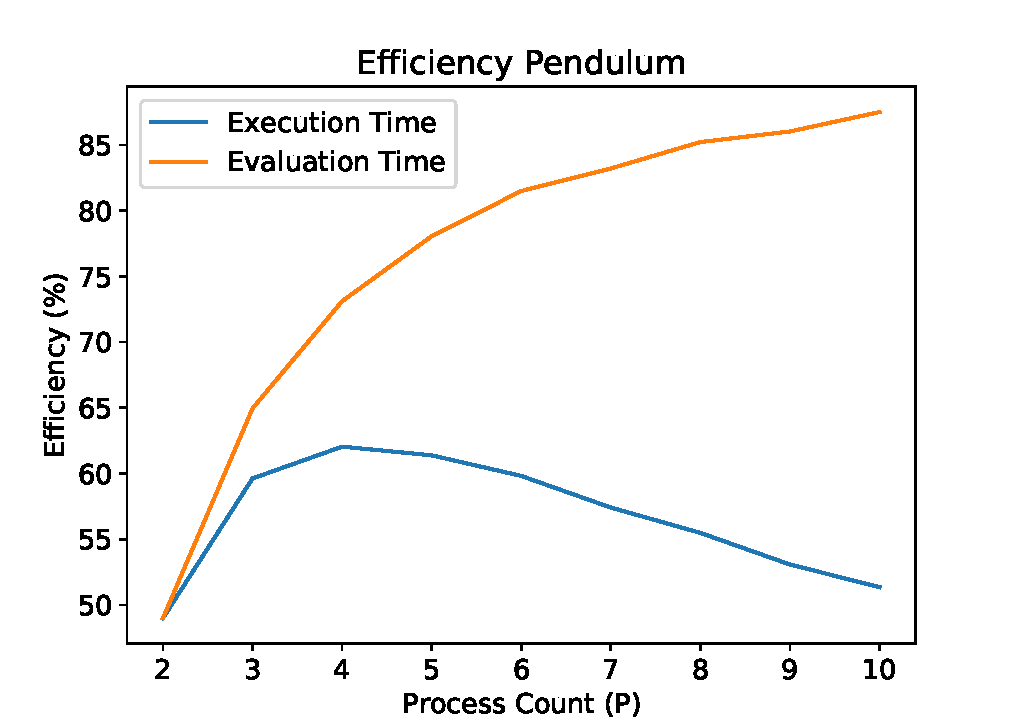
\includegraphics[width=1.0\textwidth]{./img/pendulum_analysis/efficiency_pendulum_2_10.pdf} 
	\end{minipage}
	\caption{Links der \emph{SpeedUp}, rechts die dazugehörigen Effizienzwerte für die \emph{Pendulum} Umgebung in Abhängigkeit zur Prozessanzahl}
	\label{fig:pendulum_2_10_efficiency_speedup}
\end{figure}
\\\\
Um die Ausführungszeiten und den Grad der Parallelisierung besser bewerten zu können, wird der \emph{SpeedUp} und die Effizienz für jeden Durchlauf berechnet. Die Ergebnisse sind in Abbildung \ref{fig:pendulum_2_10_efficiency_speedup} dargestellt, wobei jeweils die Werte für das gesamte Verfahren und die parallelisierte \emph{Evaluation Time} dargestellt sind. Auf Letzteres wird zuerst eingegangen. Der \emph{SpeedUp} für die Evaluationsphase ist nahezu konstant. Mit zehn Prozessen wird ein Faktor von $8.75$ erzielt. Dieses Ergebnis ähnelt dem der \emph{Mountain Car} Umgebung, bei der in dieser Phase ein Faktor von $8.7$ erreicht wird. Das Ergebnis ist insgesamt als sehr gut zu bewerten, da in der \emph{Master-Slave} Architektur mit zehn Prozessen bzw. neun \emph{Slaves} der maximal erreichbare \emph{SpeedUp} $9$ beträgt. Dies spiegelt sich auch in der Effizienz wieder. Bei der \emph{Master-Slave} Architektur liegt diese initial bei $49\%$, steigt aber stetig an. Mit zehn Prozessen wird ein Wert von $87\%$ für die Parallelisierung der \emph{Evaluation Time} erzielt. Die vergleichsweise schlechten initialen Messwerte sind durch die Berücksichtigung des \emph{Masters} bei der Berechnung zu erklären, da er selbst keine Agenten evaluiert. Derselbe Umstand tritt in der \emph{Mountain Car} Umgebung auf. Werden bei der Berechnung nur die zur Verfügung stehenden \emph{Slaves} betrachtet, liegt die Effizienz in allen Testdurchläufen bei ungefähr $97\%$, maximal bei $98\%$. Aufgrund der notwendigen Kommunikation wird keine Effizienz von $100\%$ erreicht. Zusammengefasst zeigen diese Ergebnisse, dass die Parallelisierung der \emph{Evaluation Time} in beiden Testdurchläufen sehr gute und konstante Ergebnisse liefert. Es ist davon auszugehen, dass trotz Hinzufügen von weiteren Prozessen die Effizienz bei einer entsprechenden Populationsgröße weiterhin hoch ist. Hierauf wird im Rahmen der Ergebnisse in Kapitel \ref{sec:results_optimziation} genauer eingegangen. In Abbildung \ref{fig:pendulum_2_10_efficiency_speedup} sind nicht nur der \emph{SpeedUp} und die Effizienz für die Evaluationsphase, sondern auch das gesamten Verfahrens dargestellt. Die hierbei erhaltenen Werte sind nicht so gut wie in der \emph{Mountain Car} Umgebung. Mit zehn Prozessen wird ein \emph{SpeedUp} von $5.1$ erreicht. Die \emph{Mountain Car} Umgebung erzielt im Vergleich hierzu noch einen Wert von $7.6$. Auch der Anstieg des \emph{SpeedUps} sinkt innerhalb der ersten zehn Generationen drastisch. Grund hierfür ist der Anteil der nicht parallelisierten \emph{Reproduction Time} und \emph{Compose Offspring Time}. Wie in Kapitel \ref{sec:parallel_strategies} veranschaulicht, ist in der \emph{Pendulum} Umgebung ein maximaler \emph{SpeedUp} von $11.\overline{1}$ möglich. Mit steigender Anzahl an Prozessen nähert sich das Ergebnis diesem Wert an.
\\\\
Entsprechend des \emph{SpeedUps} sind auch die Effizienzwerte weniger gut als in der \emph{Mountain Car} Umgebung. Anfangs liegt diese bei$42\%$, steigt danach an, erreicht mit vier Prozessen das Maximum von $62\%$ und sinkt danach kontinuierlich. Hierfür sind dieselben Gründe maßgeblich wie in der \emph{Mountain Car} Umgebung. Um die erhaltenen Ergebnisse besser einordnen zu können, werden mit \emph{Amdahl's Law} die zu erwartenden Effizienzwerte berechnet. Diese sind in Abbildung \ref{fig:pendulumr_efficiency_predidction} dargestellt. Aufgrund der unterschiedlichen Skalierung an den Achsen ist nicht offensichtlich, dass die gemessenen und idealen Ergebnisse sehr ähnlich sind. Die maximal erreichbare Effizienz von ungefähr $63.5\%$ tritt ebenfalls mit vier Prozessen auf. Die übrigen Effizienzwerte für zwei bis zehn Prozesse weichen weniger als zwei Prozentpunkte vom tatsächlich erhaltenen Ergebnis ab. 
\begin{figure}[!h]
	\centering
	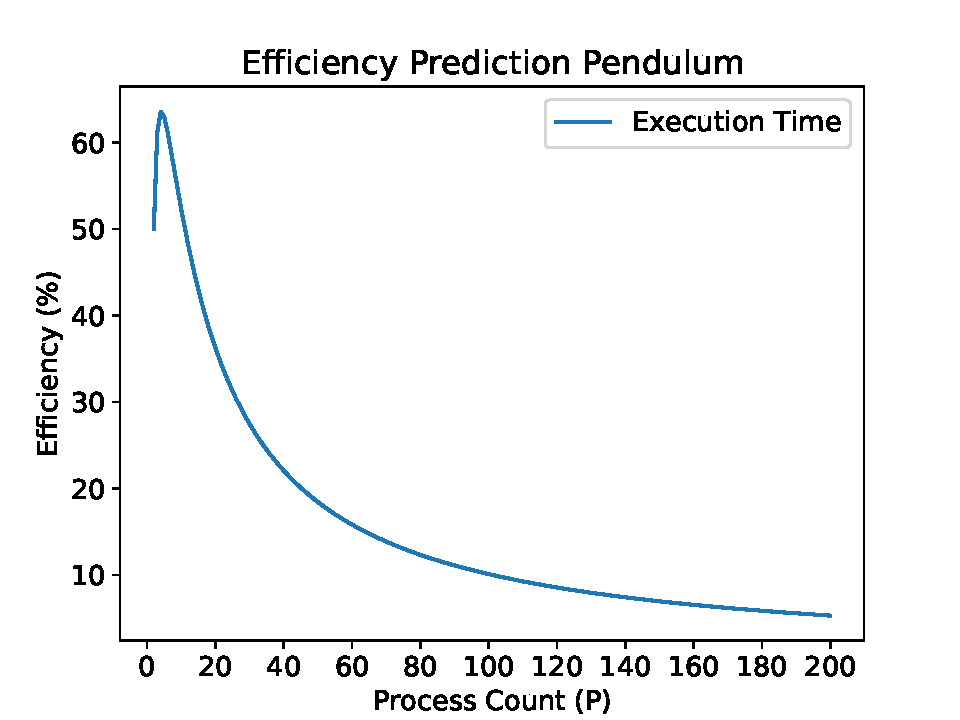
\includegraphics[width=0.7\textwidth]{./img/pendulum_analysis/pendulum_efficiency_prediction.pdf} 
	\caption{Erwartete Effizienz in der \emph{Pendulum} Umgebung in Abhängigkeit zur Anzahl an Prozessen}
	\label{fig:pendulumr_efficiency_predidction}
\end{figure}

\subsection{TITEL????}
Die bisherigen Testdurchläufe nutzen maximal zehn Prozesse gleichzeitig, einen auf jedem Raspberry Pi. Mit dieser Konfiguration werden insgesamt sehr gute \emph{SpeedUp} Ergebnisse erzielt. Prinzipiell ist es mit der bereits vorhanden Hardware möglich, die Ausführungszeit weiter zu reduzieren, da die \ac{CPU} der einzelnen Raspberry Pis nicht vollständig ausgelastet ist. Der Grund hierfür ist einerseits die Hardware und die Funktionsweise der Programmiersprache Python. In Kapitel \ref{sec:analysis_testsetup} ist beschrieben, dass der Raspberry Pi 4 über einen Quad-core ARM Prozessor verfügt. Das bedeutet, dass sich vier unabhängige Prozessoren auf derselben \ac{CPU} befinden, die parallel Programmcode ausführen können. Allerdings kann der Standard Python Interpreter dies nicht nutzen, da ein \ac{GIL} verwendet wird um die Sprache \emph{thread-safe} zu machen. Das bedeutet, dass nur ein \emph{Thread} gleichzeitig Programmcode ausführen kann. Existieren mehrere \emph{Threads} wechselt der Python Interpreter in regelmäßigen Abständen zwischen diesen, sodass jedem eine gewisse Ausführungszeit zusteht. Die Folge ist, dass alle \emph{Threads} eines Programms auf demselben Prozessor abgearbeitet werden und kein Reduzierung der Ausführungszeit möglich ist \cite{marowka2018python}. Für das Umgehen des \ac{GIL} gibt es verschiedene Ansätze, wobei eine Möglichkeit das Nutzen von \ac{MPI} ist. Die parallelisierte Implementierung kann in der vorgestellten Testumgebung auf zehn Raspberry Pis mit insgesamt $40$ Prozessen gestartet werden, sodass jeder Raspberry Pi vier Prozesse zugewiesen bekommt. Das Betriebssystem verteilt diese auf die vier verfügbaren Prozessoren und erzielt so eine parallele Ausführung. Bei dieser Umsetzung besitzen die einzelne Prozesse jeweils einen eigenen  immer noch einen eigenen \ac{GIL}, dieser interferiert jedoch mit dem von anderen Prozessen \cite{marowka2018python}.
\begin{figure}[!h]
	\centering
	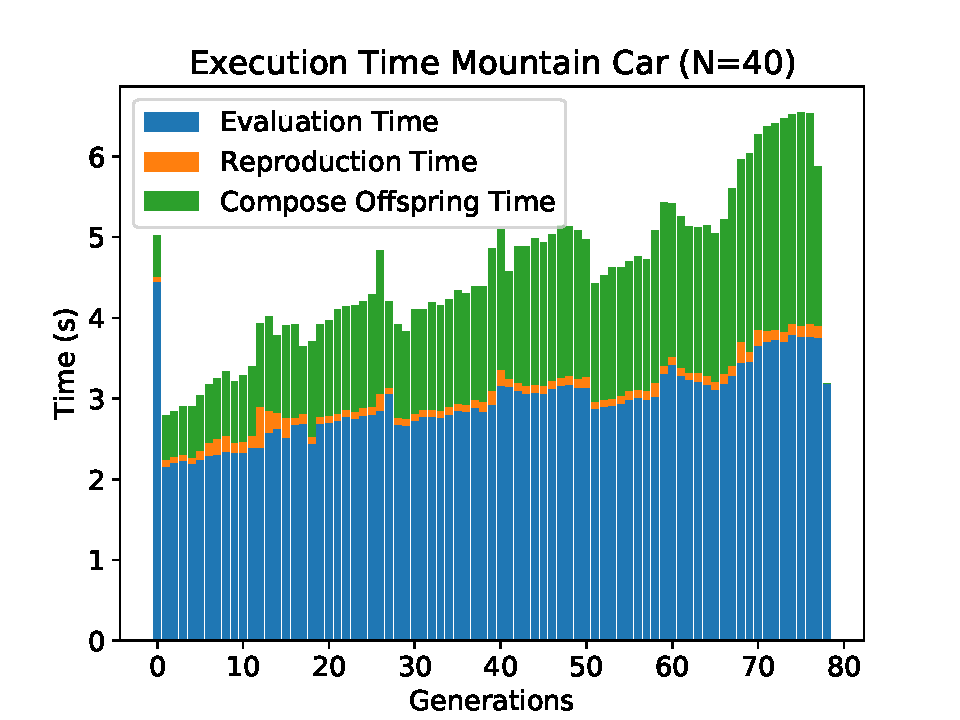
\includegraphics[width=0.7\textwidth]{./img/mountain_car_analysis/1413_time_40core_10pi.pdf} 
	\caption{Ausführungszeit des \emph{Pendulum} Problems auf 10 \emph{Raspberry Pis} mit 40 Prozessen}
	\label{fig:mountain_car_time_40core_10pi}
\end{figure}
\\\\
Um die Performance von diesem Szenario zu testen, werden die \emph{Mountain Car} und \emph{Pendulum} Umgebung erneut ausgeführt. Durch die vorherigen Ergebnisse ist zu erwarten, dass die Ausführungszeit der \emph{Evaluation Time} nahezu um den Faktor vier im Vergleich zu zehn Prozessen verringert wird. Abweichungen können durch andere Hintergrundprozesse oder das Betriebssystem entstehen, mit denen die verfügbaren Rechenkapazitäten geteilt werden müssen. Abbildung \ref{fig:mountain_car_time_40core_10pi} zeigt die gemessenen Ausführungszeiten für die \emph{Mountain Car} Umgebung mit $40$ Prozessen. Diese ist grundsätzlich im Vergleich zu den vorherigen Testdurchläufen gesunken. Insgesamt werden etwa sechs Minuten für die gesamte Ausführung benötigt, was einer Zeitersparnis von $99$ Minuten gegenüber dem sequenziellen Verfahren entspricht. Im Vergleich zu dem Testdurchlauf mit zehn Prozessen, ist die Ausführungszeit um 8 Minuten gesunken. Um eine Bewertung der Parallelisierung zu ermöglichen, wird der \emph{SpeedUp} und die Effizienz für das gesamte Verfahren sowie die \emph{Evaluation Time} berechnet.  Der \emph{SpeedUp} für das gesamte Verfahren beträgt im Vergleich zur sequenziellen Implementierung ungefähr $17.6$, die Effizienz liegt bei $44\%$. Diese Ergebnisse entsprechen nicht den Erwartungen. Nach \emph{Amdahl's Law} soll ein \emph{SpeedUp} von ungefähr $22.5$ erzielt werden, beziehungsweise von $22.1$ wenn der \emph{Master} Prozess bei der Berechnung ignoriert wird. Bei Betrachtung der \emph{Evaluation Time} sind die erhaltenen  Ergebnisse ebenfalls geringer als erwartet. Für diese Phase wird ein \emph{SpeedUp} von $26.7$ erzielt, was einer Effizienz von ungefähr $67\%$ entspricht. Selbst wenn der \emph{Master} Prozess ignoriert und nur die \emph{Slaves} betrachtet werden, liegt die Effizienz nur bei $68.4\%$. Dieses Ergebnis ist bedeutend geringer als die $97\%$ bis $99\%$, welche mit zwei bis zehn Prozessen erreichbar sind. Auch wenn bei der \emph{Pendulum} Umgebung etwas bessere Ergebnisse erzielt werden, skaliert die Leistung nicht wie erwartet. Der \emph{SpeedUp} für die \emph{Evaluation Time} beträgt ungefähr $29.6$ und ergibt eine Effizienz von $74\%$, beziehungsweise $76\%$ wenn der \emph{Master} nicht in die Berechnung miteinbezogen wird. Auch dies liegt über $20$ Prozentpunkte unter den vorherigen Ergebnissen. 
\\\\
Für den Leistungseinbruch können verschiedene Faktoren verantwortlich sein. Offensichtlich ist, dass an einer Stelle des Systems ein Ressourcenengpass entsteht. Um den Grund hierfür zu lokalisieren werden verschiedene Tests durchgeführt, auf deren Ergebnisse im Folgenden eingegangen. 

Zuerst wird der \emph{Master} Prozess untersucht. Dieser muss die Arbeitspakete mit einer geringen Latenz verteilen, sodass die \emph{Slaves} geringe Wartezeiten haben. Durch die hohe Anzahl an Prozessen, kann dies unter Umständen nicht gewährleistet werden. Um diese Behauptung zu überprüfen, wird das Optimierungsproblem angepasst. Jeder Agent muss bei der Evaluierung dieselbe Umgebung zehnmal absolvieren. Dies ändert nicht das Ergebnis, erhöhte aber die Ausführungszeit stark. Zwar ist die hierbei entstehende Last auf den \emph{Master} dieselbe, aber sie wird über eine größere Zeitspanne verteilt. Tritt bei diesem der Ressourcenengpass auf, sollte durch diese Maßnahme eine Steigerung der Effizienz erkennbar sein. Aber nach der Durchführung zeigen die Ergebnisse des Verfahrens nur eine geringfügige Steigerung. Daher kann der \emph{Master} Prozess als Engpass der Implementierung ausgeschlossen werden. 
\\\\
Stattdessen kommt die Hard- bzw. Software des Beowulf-Clusters in Frage. Um dies zu verifizieren, wird ein Testdurchlauf mit neun Prozessen und einer angepassten Konfiguration durchgeführt. Insgesamt werden drei Raspberry Pis verwendet, wobei auf einem der \emph{Master} Prozess und auf den anderen jeweils vier \emph{Slave} Prozesse gestartet werden. Mit dieser Konfiguration beträgt die Ausführungszeit des Verfahrens knapp $20$ Minuten und ein \emph{SpeedUp} von $5.3$ wird erzielt. Die \emph{Evaluation Time} macht hiervon $17.7$ Minuten aus. Diese Werte sind im Vergleich zu dem Durchlauf auf neun Raspberry Pis substanziell schlechter. Trotz derselben Anzahl an Prozessen ist die benötigte Ausführungszeit für das gesamte Verfahren $28\%$ höher und somit $4.4$ Minuten langsamer. Bei der Pendulum Umgebung treten ähnliche Ergebnisse auf. Daraus lässt sich folgern, dass sich mehrere Prozesse auf demselben Raspberry Pi teilweise gegenseitig blockieren und dadurch eine längere Ausführungszeit entsteht. 
\\\\
Zuletzt ist festzustellen, durch welche Komponenten des Algorithmus die Verzögerung entsteht. In einem ersten Schritt wird eine Umgebung des OpenAI Gyms untersucht. Abbildung \ref{fig:test_bottleneck} zeigt den erstellten Test. Es wird zuerst die \emph{Pendulum} Umgebung initialisiert und danach werden $160.000$ Zufallsaktionen ausgeführt. Die hierfür benötigte Zeit wird gemessen und am Ende ausgegeben. Der Test wird zunächst mit einem Prozess ausgeführt und hat eine gemessene Laufzeit von $75.6$ Sekunden. Danach wird der Test mit vier Prozessen auf einem Raspberry Pi wiederholt. Der zu leistende Rechenaufwand wird in diesem Fall nicht geteilt und daher sollte jeder Prozess $160.000$ Zufallsaktionen in einer lokalen Umgebung ausführen und dafür dieselbe Zeit benötigten. Allerdings zeigen die Messergebnisse einen Anstieg von $27\%$ auf $95.5$ Sekunden. Ein ähnlicher Test wird mit einem \ac{KNN} durchgeführt. Mit einem Prozess werden hierfür $73$ Sekunden benötigt. Beim der Ausführung mit vier Prozessen steigt die Laufzeit um ungefähr $9.5\%$ auf 80 Sekunden an. Da in den letzten beiden Tests keine Nachrichten ausgetauscht werden, ist zu schließen, dass die zuvor festgestellten Leistungseinbrüche mit $40$ Prozessen nicht nur einen zu großen Kommunikationsaufwand sondern vor allem durch die verwendeten Optimierungsprobleme entstehen. 
\begin{figure}
	\begin{python}
		import gym
		import time
		
		env = gym.make("Pendulum-v0")
		env.reset()
		
		start_time = time.time()
		for _ in range(160000):
			env.step(env.action_space.sample())
		
		time_required = time.time() - start_time
		print(time_required)
	\end{python}
	\label{fig:test_bottleneck}
	\caption{Python Programmcode zum Überprüfen der Parallelisierung des OpenAI Gyms}
\end{figure} 


% Prozentsatz an Abweidung nicht parllelisierter Verfahren, 
% Zuerst Ergebnisse 10 Pis, mit Verifizierung Funktionalität und allgemeines Ergebnis
% Eingehen dass Master Pi keine Abarbeitugn übernimmt sondern nur Koordination
% Zeiten von anderen Phasen weichen ab, daher kann es zu varianzen kommen
% Allgemeine Laufzeit des Verfahrens und Laufzeit des evaluierten Verfahren anzeigen
% Vergleich mit Amdahls Law? +++++ 

% !TeX spellcheck = de_DE
\section{LunarLander}
\label{sec:lunar_lander}
Die vorherigen Kapitel beschreiben die Ergebnisse des parallelisierten Verfahrens. Mit $40$ Prozessen wird ein \emph{SpeedUp} für die \emph{EvaluationTime} von $26.7$ und $29.6$ gemessen. Allerdings erfüllen die in diesen Umgebungen optimierten \ac{KNN} nicht die Eigenschaft der Generalisierung. Jedes \ac{KNN} beginnt die Evaluation immer in derselben Startposition und erzielt mit dieser gute Optimierungsergebnisse. Wenn diese \ac{KNN} in einer Umgebung mit einer abweichenden Startposition starten, besteht eine hohe Wahrscheinlichkeit, dass nicht das gewünschte Ergebnis erreicht wird. Bei der durchgeführten Analyse wird keine generelle Lösung für alle Startpositionen benötigt. Diese wäre zudem aufgrund der hohen Trainingszeiten ungeeignet. In diesem Kapitel wird ein letztes Optimierungsproblem aus dem \emph{OpenAI Gym} mit dem Namen \emph{Lunar Lander} vorgestellt. Dieses Beispiel zeigt, wie eine generelle Lösung für alle Startsituation entwickelt werden kann und die hierfür benötigten Laufzeiten. 
Das Verfahren wird ausschließlich mit dem parallelisierten Algorithmus durchgeführt. Mit den zuvor gemessenen \emph{SpeedUp} Werten kann jedoch auf die Laufzeit des sequenziellen Verfahrens geschlossen werden.
\begin{figure}[!h]
	\centering
	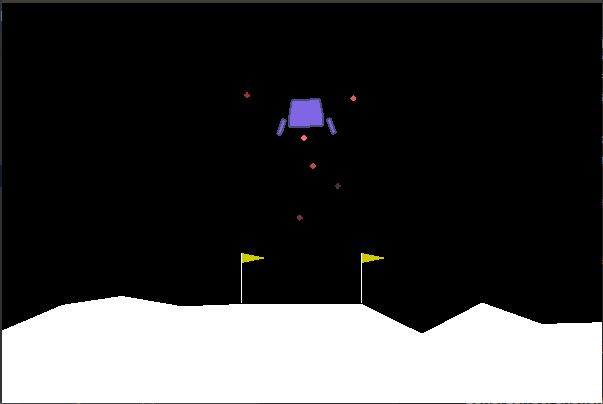
\includegraphics[width=0.5\textwidth]{./img/lunar_lander_env.JPG} 
	\caption{Darstellung der \emph{LunarLander} Umgebung aus dem \emph{OpenAI Gym}}
	\label{fig:lunar_lander_env}
\end{figure} 
\\\\
Abbildung \ref{fig:lunar_lander_env} zeigt ein Raumschiff und eine Landeplattform, die sich zwischen zwei Fahnen befindet. Ziel der Umgebung ist das Landen des Raumschiffs auf der Plattform. Für das Optimierungsproblem stehen insgesamt $8$ Eingabewerte zur Verfügung, welche die Position, Geschwindigkeit und den Winkel des Raumschiffs beschreiben. Die Koordinaten der Landeplattform sind nicht enthalten, da sich diese immer an derselben Position befindet. Als Aktion kann entweder die sich unten am Raumschiff befindende Hauptdüse oder eine Steuerdüse an der linken oder rechten Seite des Raumschiffs aktiviert werden. Ebenfalls ist es möglich, den Antrieb nicht zu aktivieren und Treibstoff zu sparen. Die Simulation der Umgebung wird beendet, wenn das Raumschiff entweder abstürzt oder erfolgreich landet. Wie bei den anderen Umgebungen des \emph{OpenAI Gyms} wird für jeden Zeitschritt ein \emph{reward} vergeben. Diese werden während der Simulation summiert und bilden den Fitnesswert. Ein positiver \emph{reward} wird vergeben, wenn das Raumschiff sinkt und sich der Plattform nähert. Zusätzlich gibt es einen Bonus, wenn das Raumschiff sich im Ziel befindet oder die Landefüße den Boden berühren. Für jeden Zeitschritt, in dem ein Antrieb aktiviert ist, wird ein kleiner Betrag vom \emph{reward} subtrahiert. Somit muss für die Maximierung des Fitnesswertes das Raumschiff so wenig Treibstoff wie möglich verbrauchen. Im Falle eines Absturzes gibt es einen negativen \emph{reward}.
\\\\
Für die Optimierung werden die Parameter der \emph{Pendulum} Umgebung übernommen. Somit steht eine Population von $1000$ Agenten zur Verfügung. Jedes \ac{KNN} besitzt entsprechend der Ein- und Ausgabewerte acht \emph{Input}- und vier \emph{Output}-Neuronen. Das Optimierungsproblem ist so konfiguriert, dass jeder Startzustand zufällig gewählt wird. Um eine generelle Lösungsstrategie zu finden, muss jeder Agent zehn Durchläufe in der Umgebung absolvieren. Für den finalen Fitnesswert werden die Ergebnisse der einzelnen Durchläufe summiert. Das Verfahren wird beendet, wenn ein Agent in jedem der zehn Durchläufe einen Fitnesswert von über $200$ Punkten erreicht. So ist sichergestellt, dass der Agent auf verschiedene Startsituationen entsprechend reagieren kann.
\begin{figure}[!h]
	\centering
	\begin{minipage}[]{0.49\textwidth}
		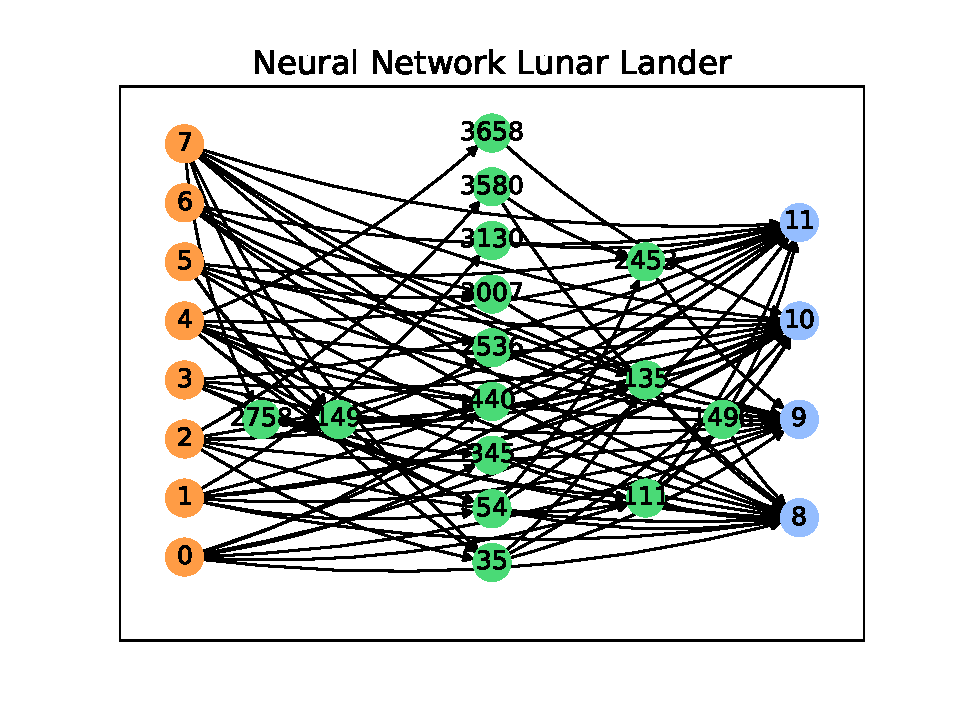
\includegraphics[width=1.0\textwidth]{./img/lunar_lander/lunar_lander_network.pdf} 
	\end{minipage}
	\hfill
	\begin{minipage}[]{0.49\textwidth}
		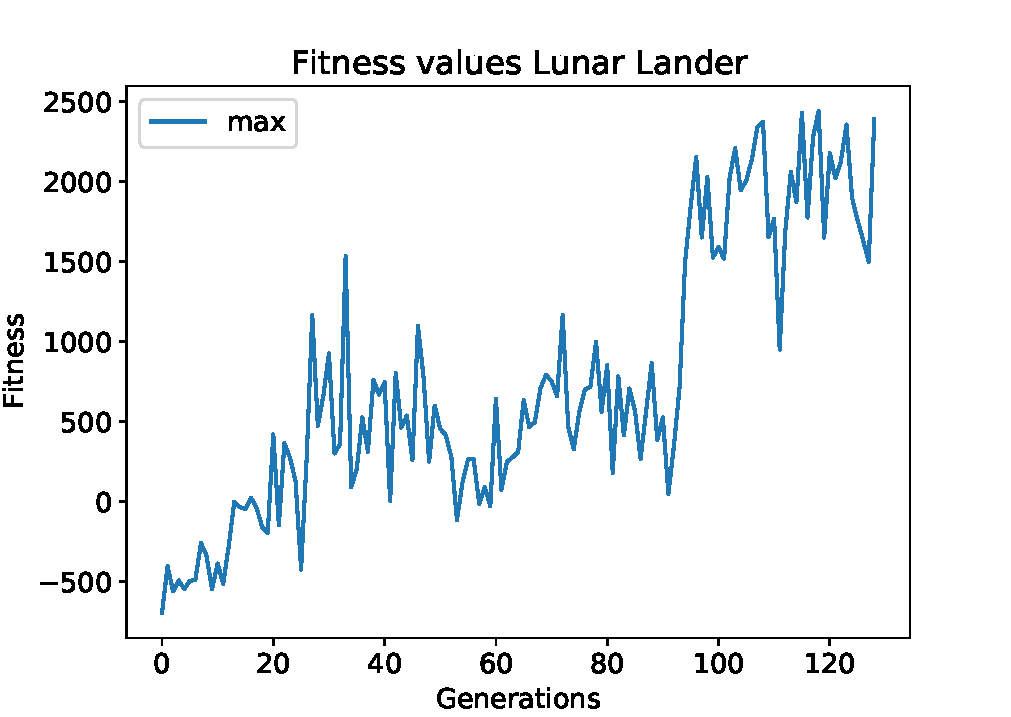
\includegraphics[width=1.0\textwidth]{./img/lunar_lander/lunar_lander_fitness.pdf} 
	\end{minipage}
	\caption{Links die Lösung für das \emph{LunarLander} Problem, rechts die dazugehörigen Fitnesswerte pro Generation}
	\label{fig:lunar_lander_neural_network_and_fitness}
\end{figure}
Abbildung \ref{fig:lunar_lander_neural_network_and_fitness} zeigt das finale \ac{KNN} und den Verlauf des maximalen Fitnesswertes. Das \ac{KNN} hat $15$ \emph{Hidden}-Neuronen entwickelt und besitzt insgesamt $88$ Verbindungen. Die Fitnesswerte sind anfänglich negativ, da das Raumschiff häufig abstürzt. Im weiteren Verlauf steigt der Fitnesswert zwar an, zeigt aber große Schwankungen aufgrund einer verrauschten Fitnessfunktion. Der Grund hierfür ist, dass nicht alle, sondern nur ein Teil der Startzustände evaluiert werden. So kann ein Agent hohe Fitnesswerte aufgrund günstiger Startpositionen erhalten, wie es zum Beispiel in Generation $33$ geschehen ist. In dieser hat der beste Agent einen Fitnesswert von $1533$ Punkten erzielt. Obwohl er unverändert in die nächste Generation kopiert wird, sinkt der maximale Fitnesswert auf $88$ Punkte. In Generation $94$ wird ein große Steigerung des Fitnesswertes auf $1495$ Punkte erzielt. Das Verfahren endet nach 128 Generationen mit einem Fitnesswert von $2394$ Punkten. Eine Besonderheit ist, dass der maximale Fitnesswert von $2441$ Punkten nicht am Ende des Verfahrens, sondern in Generation $118$ erzielt wird. 
Da jedoch die Abbruchbedingung nicht erfüllt ist, wird das Verfahren fortgeführt. Bei der Visualisierung des final entwickelten \ac{KNN} wird ersichtlich, dass das Verfahren grundsätzlich erfolgreich ist. Der Agent landet in vielen Fällen direkt auf der Zielplattform und erreicht Fitnesswerte zwischen $240$ bis $280$ Punkten. Allerdings gibt es auch Durchläufe, in denen der Agent abdriftet. In diesen Fällen landet das Raumschiff nicht auf der Plattform, dennoch werden Fitnesswerte von ungefähr $200$ Punkten erreicht. Insgesamt hat das Optimierungsverfahren eine generelle Lösungsstrategie entwickelt, aber die erreichten Fitnesswerte können aufgrund der unterschiedlichen Startpositionen dennoch abweichen. Eine bessere Leistung kann durch die Evaluation von weiteren Startzuständen oder eine höhere Trainingszeit erzielt werden.
\begin{figure}[!h]
	\centering
	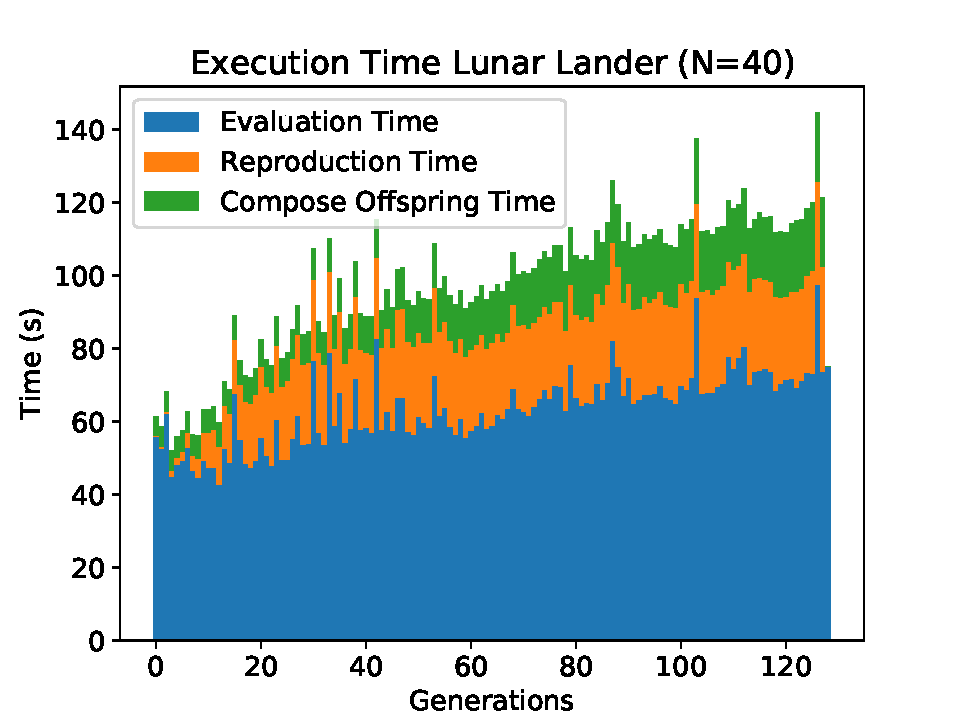
\includegraphics[width=0.9\textwidth]{./img/lunar_lander/lunar_lander_time_40.pdf} 
	\caption{Ausführungszeit des \emph{LunarLander} Problems auf 10 Raspberry Pis mit 40 Prozessen}
	\label{fig:lunar_lander_time_40core_10pi}
\end{figure}
\\\\
Abbildung \ref{fig:lunar_lander_time_40core_10pi} zeigt die gemessenen Ausführungszeiten mit $40$ Prozessen auf zehn Raspberry Pis. Insgesamt hat das Verfahren etwa $3.5$ Stunden benötigt. Hiervon werden ungefähr $65\%$ für die \emph{Evaluation Time} verwendet. Der zweitgrößte Faktor der Ausführungszeit ist die \emph{Reproduction Time} mit ungefähr $22\%$, welcher wie bei der \emph{Pendulum} Umgebung durch die vielen verschiedenen Spezies zu erklären ist. Wie bei der \emph{MountainCar} Umgebung unterliegt die Ausführungszeit der einzelnen Generationen einigen Schwankungen, da die Evaluationszeit je nach Agent stark abweichen kann. Stürzt das Raumschiff direkt ab oder landet schnell, ist die Evaluationszeit kurz. Evaluationen mit einer hohen Flugzeit können hingegen vergleichsweise lange andauern. Auch die Größe des \ac{KNN} kann ein entscheidender Faktor sein, sowohl bei der \emph{Evaluation} als auch in den Phasen \emph{Mutation} und \emph{Rekombination}. Um in solchen Szenarien gute Effizienzwerte zu erhalten, ist die dynamische Zuteilung von Arbeitspaketen durch die \emph{Master-Slave} Architektur besonders wichtig. Prinzipiell hätte diese Umgebung auch bei der Analyse in Kapitel \ref{chap:analysis} verwendet werden können, die lange Ausführungszeit ist jedoch nicht praktikabel. Mit den \emph{SpeedUp} Werten aus der \emph{MountainCar} und \emph{Pendulum} Umgebung ist auf die sequenzielle Ausführungszeit zu schließen. Bei einem \emph{SpeedUp} Faktor von $26.7$ bzw. $29.6$ liegt die erwartete Ausführungszeit zwischen $62.1$ und $68.7$ Stunden. 
% !TeX spellcheck = de_DE
\section{Ergebnisse}
\label{sec:results_optimziation}
Auf Basis der Analyse ist das parallelisierte Verfahren implementiert und danach getestet worden. Die hierbei erhaltenen Ergebnisse sind im Folgenden zusammengefasst. Der größte Einfluss bezüglich der Ausführungszeit ist die \emph{Evaluation Time}, welche in beiden Verfahren über $90\%$ ausmacht. Somit kann durch eine Parallelisierung dieser Phase die größte Zeiteinsparung erzielt werden. \emph{Amdahl's Law} zeigt, dass durch den sequenziellen Anteil de Programmcodes, trotz unendlich vieler Prozesse ein maximaler \emph{SpeedUp} von $50$ für die \emph{Moutain Car} Umgebung und von $11.\overline{1}$ für die \emph{Pendulum} Umgebung möglich ist. Diese Werte werden für einen Vergleich mit den tatsächlich erhaltenen Ergebnissen genutzt.
\\\\
Für eine maximale Zeitersparnis wird die Evaluation der Agenten als ganzes parallelisiert. Ein Vorteil ist, dass sowohl das Optimierungsproblem als auch die Funktionalität des \ac{KNN} parallel ausgeführt werden. Zusätzlich ist bei dieser Umsetzung der entstehende Kommunikationsaufwand gering und das nachträgliche Integrieren von Bibliotheken wie Tensorflow und PyTorch ist möglich. Für die eigentliche Implementierung sind verschiedene Anforderungen definiert, die vollständig umgesetzt sind. Es wird eine \emph{Master-Slave} Architektur für die Kommunikation verwendet. Diese ist einfach zu implementieren, vermeidet \emph{Deadlocks} und ermöglicht eine dynamische Lastenverteilung. Letzteres ist besonders wichtig, wenn das parallelisierte Verfahren auf unterschiedlich leistungsfähigen Geräten ausgeführt wird oder sich die Evaluationszeit von Agenten unterscheidet. Ein Nachteil dieser Umsetzung ist, dass der \emph{Master} nur die Koordination der Kommunikation übernimmt und die \emph{Slaves} nicht bei der Evaluation unterstützt. In der Effizienzberechnung macht dies bei einer geringen Anzahl an Prozessen einen großen Unterschied. In größeren Systemen mit hunderten Prozessen hingegen ist der Einfluss vernachlässigbar gering und daher nicht relevant. Bei der Implementierung des parallelisierten Verfahren werden die Komponenten des sequenzielle Verfahrens überwiegen wiederverwendet. Hierdurch ist eine schnelle und effiziente Entwicklung möglich. Entscheidend ist, dass beide Verfahren einfach untereinander austauschbar sind und ein direkter Vergleich ermöglicht wird. Um letzteres zu gewährleisten, basiert auch das parallelisierte Verfahren auf einem \emph{Seed}. Ist dieser identisch wie beim sequenziellen Verfahren, werden dieselben Ergebnisse berechnet. Für die Kommunikation wird der Standard \ac{MPI} eingesetzt, da er im Bereich \ac{HPC} weit verbreitet ist und zusätzlich das Umgehen des \acp{GIL} von Python ermöglicht.
\\\\
Für die Tests wird ein Beowulf Cluster bestehend aus zehn Raspberry Pis erstellt. Auf diesem wird das parallelisierte Verfahren durchgeführt und mit den Laufzeiten des sequenziellen verglichen. Anfänglich wird das Verfahren jeweils mit einem Prozess pro Raspberry Pi durchgeführt. Insgesamt sind die hierbei erhaltenen Werte für den \emph{SpeedUp} und die Effizienz nur geringfügig niedriger als durch \emph{Amdahl's Law} vorhergesagt. Mit zehn Prozessen wird für das gesamte Verfahren ein \emph{SpeedUp} von $7.6$ bzw. $5.1$ für die \emph{Mountain Car} und \emph{Pendulum} Umgebung erzielt. Da diese Werte durch den sequenziellen Anteil des Algorithmus beeinflusst sind, wird die parallelisierte \emph{Evaluation Time} gesondert bewertet. Mit zehn Prozessen liegen die erzielten \emph{SpeedUp} Werte bei $8.5$ und $8.7$. Werden nur die \emph{Slaves} bei der Berechnung der Effizienz berücksichtigt, beträgt diese in jedem Testdurchlauf mindestens $97\%$. Das verdeutlicht die Effizienz der Kommunikation und den Erfolg der Parallelisierung.
\\\\
Mit \ac{MPI} ist es möglich das \ac{GIL} von Python zu umgehen. Damit kann das parallelisierte Verfahren alle $40$ Prozessoren des erstellten Beowulf Clusters vollständig auslasten. Zwar ist das Verfahren grundsätzlich schneller als mit zehn Prozessem, allerdings skaliert der \emph{SpeedUp} entgegen den Erwartungen in diesem Fall nicht so gut. Verschiedene Tests veranschaulichen, dass dies nicht durch die höhere Anzahl von beteiligen Prozessen entsteht. Diese Erkenntnis ist entscheidend, wenn der Algorithmus in größeren und leistungsfähigeren Clustern ausgeführt werden soll. Stattdessen ist auf Basis der durchgeführten Tests zu schlussfolgern, dass sich mehrere Prozesse auf demselben Raspberry Pi gegenseitig blockieren. Dieses Phänomen ist unabhängig von der Anzahl der beteiligten Prozesse. Um die genaue Ursache hiervon festzustellen, sind weitere Tests notwendig, die nicht Teil dieser Arbeit sind. Ein möglicher Ressourcenengpass kann beispielsweise beim Zugriff auf Systemressourcen wie den \ac{RAM} entstehen. Ist die hierfür bereitgestellte Bandbreite nicht ausreichend für alle vier Prozessoren gleichzeitig, wird es zu Verzögerungen und somit niedrigeren \emph{SpeedUp} Werten kommen. 
\\\\
Die zuletzt vorgestellte \emph{Lunar Lander} Umgebung dient als Beispiel, wie eine generelle Lösungsstrategie entwickelt werden kann. Im Vergleich zu den vorherigen Umgebungen verwendet diese zufällige Startzustände und das \ac{KNN} muss lernen auf diese zu reagieren. Dies ist anspruchsvoller, als nur eine Lösung für einen einzelnen Startzustand zu entwickeln. Hierbei ist ein grundsätzliches Problem, dass die Fitnessfunktion nicht alle Startzustände miteinbezieht. Schlechte \ac{KNN} können mit einfachen Startzuständen gute Fitnesswerte erzielen und vielversprechende \ac{KNN} in schwierigen Umgebungen niedrige. Die hieraus entstehende Gefahr ist, dass vielversprechende Lösungsansätze durch niedrige Fitnesswerte bei der Selektion nicht ausgewählt werden und verloren gehen. Um dies zu verhindern und einen aussagekräftigen Fitnesswert zu erhalten, wird in diese Beispiel die Umgebung zehnmal nacheinander mit unterschiedlichen Startzuständen evaluiert. Erst wenn für jeden Durchlauf eine gültige Lösungsstrategie gefunden ist, wird das Verfahren beendet. Wie in dem Beispiel gezeigt, ist das Vorgehen erfolgreich. Der große Nachteil ist, dass die Evaluationszeit stark erhöht wird. Hierbei zeigt sich der große Vorteil der Parallelisierung. Mit den zuvor gemessenen \emph{SpeedUp} Werten wird angenommen, dass die Ausführungszeit mit dem sequenziellen Verfahren zwischen $62.1$ und $68.7$ Stunden benötigt hätte. In der parallelisierten Umgebung hingegen, wird das Verfahren bereits nach $3.5$ Stunden beendet. Es ist davon auszugehen, dass durch Hinzufügen von weiteren Prozessoren die Ausführungszeit entsprechend \emph{Amdahl's Law} weiter gesenkt werden kann. Dieses Beispielproblem verdeutlicht erneut den Erfolg der Parallelisierung.


